\documentclass[letterpaper,journal]{IEEEtran}

% IEEE Transactions journal template packages, with additions used in this paper.
\usepackage{amsmath,amsfonts,amssymb}
\usepackage{algorithmic}
\usepackage{algorithm}
\usepackage{array}
\usepackage{booktabs}
\usepackage[caption=false,font=normalsize,labelfont=sf,textfont=sf]{subfig}
\usepackage{textcomp}
\usepackage{stfloats}
\usepackage{url}
\usepackage{verbatim}
\usepackage{graphicx}
\usepackage{cite}
\usepackage[hidelinks]{hyperref}
% Allow figures and tables to share pages with text instead of float-only pages.
\setcounter{topnumber}{4}
\setcounter{dbltopnumber}{3}
\renewcommand{\topfraction}{0.90}
\renewcommand{\dbltopfraction}{0.90}
\renewcommand{\textfraction}{0.05}
\renewcommand{\floatpagefraction}{0.80}
\renewcommand{\dblfloatpagefraction}{0.80}

\title{When Image Statistics Mislead: A Reproducibility Audit of Six Chaos-Based Image Encryption Papers and Authenticated-Encryption Controls}

\author{P. Vishnu Vardhan%
\thanks{P. Vishnu Vardhan is with the Department of Computer Science, SRM University AP, Amaravati 522240, Andhra Pradesh, India (e-mail: \href{mailto:vishnuvardhan_p@srmap.edu.in}{\texttt{vishnuvardhan\_p@srmap.edu.in}}; ORCID: \href{https://orcid.org/0009-0007-5130-4011}{0009-0007-5130-4011}).}}

\begin{document}
\maketitle

\begin{abstract}
Recent image-encryption papers often treat entropy, histograms, correlation, and NPCR/UACI as security evidence, although these statistics do not test whether an attacker can recover information or alter a message undetected. We review six recent chaos-based image-encryption papers and evaluate AES-256-GCM and ChaCha20-Poly1305 controls on 22 USC-SIPI images. All 44 image cases round-tripped exactly, and all 572 corruption or wrong-key probes were rejected. With fresh nonces, NPCR/UACI were nearly identical for unchanged and one-byte-changed plaintexts. An equation-level audit of Zhang et al.'s bit-plane diffusion found a chosen-input collision: complementing the first bit sequence leaves the published cyclic-XOR diffusion output unchanged. The collision held in all 65,536 exhaustive assignments at sequence length four, in 500/500 seeded synthetic probes, and for 12/12 grayscale benchmark images under the paper's example bit-plane grouping. Further audits found a zero denominator in 161/10,000 Geng input variants, a negative radicand in at least one printed Zhu equation for 75.00\% of one million sampled inputs, and plaintext-dependent Niu initial states under an explicit byte-serialization assumption. These are bounded equation findings; no full target cipher or quantum circuit has been reproduced.\end{abstract}

\begin{IEEEkeywords}
image encryption, chaos-based cryptography, authenticated encryption, reproducibility, security evaluation, chosen-plaintext input, NPCR, UACI
\end{IEEEkeywords}

\section{Introduction}
\IEEEPARstart{D}{igital} images are used in health care, remote sensing, industry, and personal communication. Their large size and spatial structure have motivated many image-encryption designs based on chaotic maps, bit-plane operations, DNA coding, compressed sensing, and pixel permutation. Six recent examples considered here combine these ingredients in different ways \cite{niu2024,zhang2024,zhu2024,yan2025,geng2025,aldayel2025}.

The papers report a wide range of experiments, including entropy, histograms, adjacent-pixel correlation, key sensitivity, NPCR/UACI, noise tests, and chaotic-system analyses. These are useful diagnostics. However, a high ciphertext entropy or a large NPCR does not establish resistance to a chosen-plaintext attack, and a successful image round trip does not establish ciphertext integrity. The security question depends on the attacker, the key and nonce rules, and the exact encryption/decryption implementation.

This work has three limited aims. First, it maps the evaluation procedures reported in the six supplied papers to reproducible control tests using established authenticated-encryption algorithms. Second, it audits published equations from Niu et al., Geng et al., and Zhu and Zhu for input dependence, undefined values, and non-real outputs. Third, it records which missing implementation details prevent end-to-end cipher reproduction. The control tests do not reproduce the six ciphers.

The contributions of this draft are:
\begin{itemize}
  \item a paper-by-paper inventory of reported tests and the additional implementation details needed for independent reproduction;
  \item a mode-preserving control evaluation of AES-256-GCM and ChaCha20-Poly1305 on 22 grayscale and RGB research images, including integrity, wrong-key, image-statistic, and timing measurements; and
  \item a chosen-input collision and decryption-correctness failure in Zhang et al.'s published cyclic-XOR diffusion, alongside reproducible equation audits of Niu, Geng, Zhu, and Yan, with each result scoped to the equations actually analyzed.
\end{itemize}

This draft does not propose a new cipher or claim key recovery or plaintext recovery against any of the six schemes. The Zhang equation audit does establish a non-injective mapping and a correctness failure under the stated deterministic equations, but is not a full cipher reproduction. These limits matter for the intended venue. IEEE Transactions on Information Forensics and Security (TIFS) covers information security and encourages reproducibility, but the current evidence is not yet a complete cipher-specific security contribution \cite{tifsScope}. The target venue must be reassessed after the remaining experiments.

\section{Related Work and Evaluation Scope}
The six papers cover several different designs. Niu et al. combine an improved four-dimensional chaotic system with evolutionary operators \cite{niu2024}. Zhang et al. present non-equal-length image encryption using bit-plane chaotic mapping \cite{zhang2024}. Zhu and Zhu combine visual-security embedding, multi-key selection, compressed sensing, and a four-dimensional map \cite{zhu2024}. Yan et al. use a conservative chaotic system and DNA operations for color images \cite{yan2025}. Geng et al. combine a Thorp shuffle, pseudo-dequeue operations, and bit-plane diffusion \cite{geng2025}. Al-Dayel et al. combine a four-dimensional chaotic system and a cellular automaton \cite{aldayel2025}. Recent related work by coauthors of this manuscript studies lightweight 2D chaos for UAV image communication and a hybrid chaos-based image-sharing design \cite{bhargav2025lightweight,molika2026sharing}. These application-oriented studies motivate reporting both computational measurements and integrity behavior; they are cited here as related work, not treated as members of the six-paper audit set.

Foundational chaos-based cryptography papers explain why a visual appearance of randomness is not a cryptographic argument: early designs used low-dimensional maps and iterative permutation/substitution \\cite{fridrich1998,kocarev2001}, while later work documented finite-precision degradation and requirements for key management, implementation, and attack analysis \\cite{lidynamics2005,alvarezli2006,jakimoski2001}. Chosen- and known-plaintext analyses have repeatedly demonstrated weaknesses in particular chaos-based image schemes \\cite{chaoticcryptanalysis2002,cokalsolak2009,liimage2009,liFridrich2017,lientropy2018,zhuzhu2021bitplane,deng2025}. These precedents motivate a paper-specific coverage matrix; they do not establish that any of the six current targets is broken. Surveys summarize the range of chaos-based designs and evaluation choices \\cite{li2019review,zia2022survey,fang2023survey,zhangliu2023review,comprehensivesurvey2024}.

Image entropy and differential-image statistics are useful descriptive measurements, and prior work proposed image-oriented randomness measures \\cite{shannon1949,wu2011entropy}. They must be interpreted within an attacker model: differential cryptanalysis is defined by controlled input differences and output observations \\cite{bihamshamir1991}, not by a single plaintext-to-ciphertext comparison. NIST explicitly cautions that statistical tests cannot certify cryptographic suitability or replace cryptanalysis; NIST later announced that SP 800-22 would be revised to clarify that it should not assess cryptographic random number generators \\cite{nistSP80022,nistSP80022decision}.

For the control algorithms, AES is standardized in FIPS 197, while GCM and other block modes are specified by NIST recommendations; AEAD interfaces and their confidentiality/integrity intent are also standardized in RFC 5116 \\cite{nistFIPS197,nistSP80038A,rfc5116,bellarenamprempre2008}.

Their evaluation procedures are not interchangeable. Some focus on chaotic dynamics or NIST sequence tests; others emphasize image statistics, key sensitivity, noise/cropping recovery, or simulation. A test can only be reproduced fairly when the equations, numerical precision, image preprocessing, test parameters, and timing boundary are known. Our inventory records the published procedures and labels tests of standard AEAD controls separately from tests that require each paper's own cipher.

This manuscript is a reproducibility audit, not a newly proposed chaos-based cipher. The phase portraits, bifurcation plots, and Lyapunov-exponent plots in the source papers characterize each paper's particular dynamical system. We do not add one as a result here because we do not independently reproduce a complete chaotic generator with its numerical solver, precision, and parameter settings. Our diagram therefore shows the study workflow, not a new encryption pipeline.

Authenticated encryption with associated data (AEAD) provides confidentiality and integrity for a message and its associated metadata. AES-GCM is specified in NIST SP 800-38D, and ChaCha20-Poly1305 is specified in RFC 8439 \cite{nistGCM,rfc8439}. These algorithms are reference controls in this work, not proposed image ciphers. Their use helps distinguish descriptive image measurements from a cryptographic integrity check.

\section{Research Questions and Threat Model}
We ask three bounded questions:
\begin{enumerate}
  \item Do image-statistic values from an authenticated-encryption control meaningfully measure confidentiality or integrity?
  \item Do basic ciphertext changes, metadata changes, truncation, or wrong keys pass through the AEAD control?
  \item What input-dependent or undefined behavior is directly reproducible from the published Niu and Geng seed equations, and what information is missing for end-to-end reproduction?
\end{enumerate}

For the AEAD controls, the evaluator can view the public image mode and dimensions, change ciphertext or authenticated metadata, truncate the container, and submit a wrong key. The evaluator does not attempt key recovery, exploit a cipher implementation, or obtain a decryption oracle beyond checking that invalid messages fail authentication. The pixel-change comparison is a diagnostic experiment, not a formal chosen-plaintext attack on AES-GCM or ChaCha20-Poly1305.

For the equation audits, the evaluator knows the published formula and can choose image inputs. The measured outcomes are limited to schedule changes, undefined arithmetic, or non-real values under the stated inputs. These probes do not claim plaintext or secret-parameter recovery.

\section{Methods}
The study follows two parallel paths: a source-paper review with bounded equation audits, and a separate authenticated-encryption control evaluation on a 22-image corpus. Figure~\ref{fig:workflow} summarizes these paths and their synthesis. The control ciphers are not implementations of the six reviewed methods.

\begin{figure*}[!t]
\centering
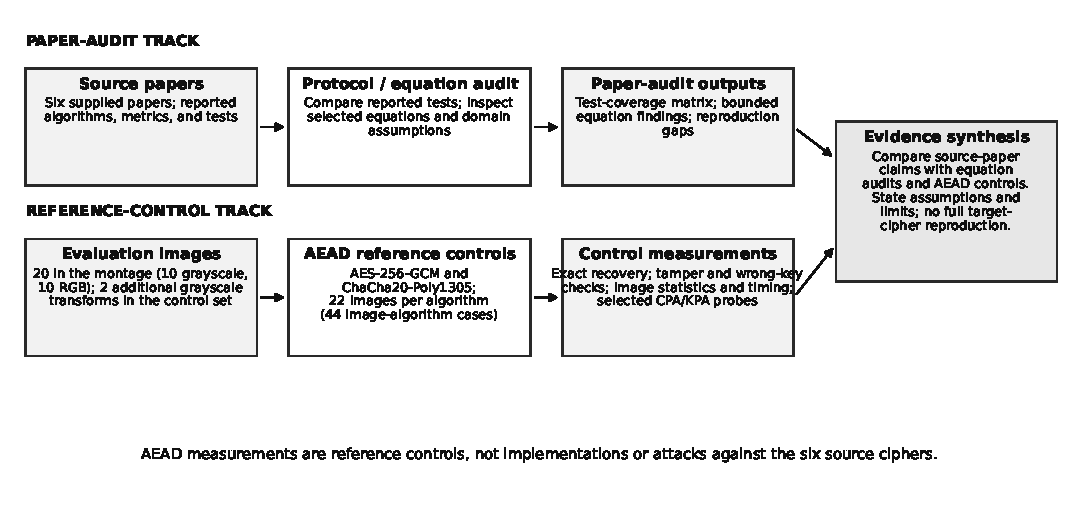
\includegraphics[width=0.96\textwidth]{figures/methodology_overview.pdf}
\caption{Two-track study design. The upper track reviews six supplied papers and performs bounded audits of selected equations. The lower track evaluates AES-GCM and ChaCha20-Poly1305 reference controls on 22 image assets; 20 are shown in the montage and two are derived grayscale transforms. The tracks are synthesized with their assumptions and limits kept explicit. The reference controls are not implementations of or attacks against the six source ciphers.}
\label{fig:workflow}
\end{figure*}
\subsection{Image Corpus and Reference Implementations}
We used 22 TIFF images from the USC-SIPI Image Database: 10 original grayscale images, 10 original RGB images, and two grayscale transformations of RGB images for paired checks. The per-image manifest records source identifier, dimensions, transformation, and SHA-256 hash. Figure~\ref{fig:image-montage} displays the 10 original grayscale and 10 original color images used in the benchmark. The database is intended for research, but USC-SIPI notes that copyright is unknown for many images; reproduction permission for the displayed panels must be confirmed before journal submission \cite{uscSipi,uscSipiCopyright}.

The baseline used AES-256-GCM and ChaCha20-Poly1305 with 32-byte keys, fresh cryptographic 96-bit nonces, and 128-bit authentication tags. A canonical JSON header containing the algorithm, image dimensions, pixel mode, data type, and format version was authenticated as associated data. Each of the 22 assets was tested with both algorithms, for 44 image--algorithm cases. The recorded run used Windows 11, Python 3.12.14, Pillow 13.0.0, NumPy 2.5.4, and cryptography 50.0.2 on an AMD64 system; exact image hashes and per-run outputs are included in the supplement. We checked exact pixel recovery, ciphertext/tag bit changes, a metadata edit, central occlusions at three areas, salt-and-pepper corruption at four densities, one-byte truncation, a random wrong key, and a one-bit wrong-key change. The 13 integrity/key probes per case produced 572 total probes. The example panels use color images 15 and 16 in the paper's numbering; their original source identifiers remain in the data manifest. The USC-SIPI copyright page identifies these two USC jelly-bean photographs as free to use \cite{uscSipiCopyright}.

As a separate nonce-lifecycle control, we reanalyzed a six-image NASA pilot using both reference algorithms (12 image-algorithm cases). For each case, the harness compared ciphertext bodies for (i) identical plaintexts encrypted under independent fresh nonces, (ii) a one-byte-changed plaintext under a fresh nonce, and (iii) a one-byte-changed plaintext under the same key and nonce. The third condition is deliberately unsafe and was isolated from all normal benchmark runs. We also checked whether XOR of the two ciphertext bodies equals XOR of their plaintexts. This illustrates nonce misuse in the reference stream-encryption modes; it is not an attack on any of the six supplied image ciphers.

\subsection{Image Diagnostics and Timing}
For each ciphertext body, we measured byte and channel entropy, adjacent-pixel correlation, local entropy, histogram chi-square, and Fourier-spectrum summaries. For a byte-valued array $X$, empirical entropy is $H(X)=-\sum_{v=0}^{255}p(v)\log_2p(v)$. For two aligned arrays $X,Y$ of $N$ bytes, we compute $\mathrm{NPCR}(X,Y)=100N^{-1}\sum_i\mathbf{1}[X_i\ne Y_i]$ and $\mathrm{UACI}(X,Y)=100(255N)^{-1}\sum_i|X_i-Y_i|$. The differential table reports five independent fresh-nonce pairs per image and algorithm for both unchanged plaintext and a one-byte plaintext change. Fresh nonces randomize the stream and therefore make these image-style scores unsuitable as intrinsic-diffusion measurements; both conditions are reported to demonstrate this confound. The earlier per-image table separately shows the direct aligned plaintext-versus-ciphertext-body byte comparison and labels it descriptive. None of these statistics is treated as a security proof.

We measured in-memory encryption and decryption time using one warm-up and 30 repetitions per image-algorithm case. The reported average throughput is the arithmetic mean of the per-image throughput values in the original run. We also measured file-level sealing and opening with one warm-up and nine repetitions per case. File sealing includes image decoding and writing the authenticated container. File opening includes reading the container, authentication/decryption, and lossless PNG output at compression level 1. The measurements describe this specific Python/Windows/AMD64 environment and cannot be compared directly with the six papers' timings, which used different software, hardware, images, and timing boundaries.

For two additional color examples, we performed fresh-nonce NPCR/UACI diagnostics (30 pairs per input condition), a simple fixed-length CPA distinguisher (500 randomized challenges per algorithm), a known-plaintext cross-nonce keystream-transfer probe (100 target messages), and 100 random wrong-key trials per image-algorithm case. We also tested salt-and-pepper and Gaussian byte noise at 0.1\%, 1\%, 5\%, and 10\%, ciphertext and tag bit changes, authenticated metadata changes, truncation, and 16-byte ciphertext-block reordering. Scrambling-only attacks do not apply to this AEAD construction because it has no separate permutation layer. These are small diagnostics, not formal CPA/KPA/COA security proofs or attacks on the six custom ciphers. A timing screen compared 1,500 same-size all-zero and fixed pseudorandom messages per class and algorithm using Welch's t-test; significant and nonsignificant outcomes are both exploratory and cannot establish or rule out an exploitable timing channel. The whole-image wrapper has $O(n)$ time and $O(n)$ working memory for $n$ pixel bytes. Exhaustive search was not performed; for a 256-bit uniformly random key, the idealized average search is $2^{255}$ trials, whose wall time depends entirely on an assumed trial rate.

\begin{algorithm}[t]
\caption{Control evaluation for one image and AEAD algorithm}
\label{alg:control}
\begin{algorithmic}[1]
\REQUIRE Pixel array $P$, dimensions $(w,h)$, mode $m$, AEAD algorithm $A$
\STATE Generate a 256-bit key $K$
\STATE Encode $(w,h,m)$ as associated data $D$
\STATE $C \leftarrow \operatorname{AEAD.Enc}(K,P,D)$ using a fresh nonce
\STATE $P' \leftarrow \operatorname{AEAD.Dec}(K,C,D)$
\STATE Record whether $P'=P$
\FOR{each corruption, metadata edit, truncation, or wrong-key probe $q$}
  \STATE Apply $q$ to the container or key
  \STATE Record whether authenticated decryption rejects the result
\ENDFOR
\STATE Compute descriptive image metrics and repeated timing values
\RETURN Round-trip, rejection, metric, and timing records
\end{algorithmic}
\end{algorithm}

\begin{algorithm}[!t]
\caption{AEAD image encryption (sealing)}
\label{alg:seal}
\begin{algorithmic}[1]
\REQUIRE Image bytes $P$, dimensions $(w,h)$, mode $m$, algorithm $A$, secret key $K$
\STATE $D \leftarrow \operatorname{CanonicalHeader}(A,w,h,m,\texttt{uint8},\text{version }1)$
\STATE $N \leftarrow \operatorname{CSPRNG}(96\text{ bits})$
\STATE $(C,T) \leftarrow \operatorname{AEAD.Enc}_{K}(N,P,D)$
\STATE $E \leftarrow \texttt{IMGBEN1\textbackslash{}0} \\| \operatorname{u16}(|D|) \\| D \\| N \\| C \\| T$
\RETURN Binary container $E$
\end{algorithmic}
\end{algorithm}

\begin{algorithm}[!t]
\caption{AEAD image decryption (opening)}
\label{alg:open}
\begin{algorithmic}[1]
\REQUIRE Binary container $E$, secret key $K$
\STATE Parse magic, header length, authenticated header $D$, nonce $N$, ciphertext $C$, and tag $T$
\IF{magic, lengths, mode, or dimensions are invalid}
  \STATE Reject $E$
\ENDIF
\STATE $P \leftarrow \operatorname{AEAD.Dec}_{K}(N,C,T,D)$
\IF{authentication fails}
  \STATE Reject $E$ and return no image
\ENDIF
\STATE Reshape $P$ using the authenticated mode and dimensions
\RETURN Recovered image
\end{algorithmic}
\end{algorithm}

\subsection{Published-Equation Audits}
\subsubsection{Niu et al. Plaintext-Dependent Initial-State Schedule}
Equations (8)--(10) derive four chaotic initial values using the plaintext column means and a SHA-256 digest of the image \cite{niu2024}. We transcribed these equations with the published example base values $(0.01,0.01,0.01,0.01)$ and applied nearest-integer rounding as described in the article. The digest input is assumed to be row-major 8-bit grayscale pixel bytes because the paper does not specify its serialization. As a sensitivity check, we also computed a floor-fraction variant; this is not treated as an equally supported reading of the paper. We evaluated both variants on 12 grayscale images and on 1,000 seeded one-pixel edits of image 4.2. This is a schedule-level audit only: it does not integrate the ODE or reproduce image encryption. The publisher's data statement says generated/analyzed data are included in the article; no code-availability statement appears on the article page.

We also analyzed a chosen-plaintext equality distinguisher under the stateless interpretation of the published steps: the external initial key is fixed, each image determines its own initial state, and no fresh per-encryption nonce or randomized input is specified. For two distinct, equal-size plaintexts $P_0$ and $P_1$, the distinguisher queries $P_0$ once and receives $C_0$, then submits $(P_0,P_1)$ as the challenge pair. It guesses $P_0$ exactly when the challenge ciphertext equals $C_0$. If encryption is deterministic and correct for both messages under the fixed key, ciphertext equality occurs exactly for $P_0$, so the success probability is 1 and the usual distinguishing advantage is $1/2$. This is a formal equality-leakage result under the stated interpretation; it does not recover pixel values or the secret key. A specified per-message state or nonce could change the conclusion, but none is described in the published algorithm.

\subsubsection{Zhang et al. Cyclic-XOR Diffusion Collision}
We transcribed the binary diffusion in Eqs. (11)--(16) from the supplied PDF \cite{zhang2024}. For a length-$L$ bit sequence, define $D(x)_1=x_1\oplus x_L$ and $D(x)_i=x_i\oplus x_{i-1}$ for $i>1$. Eqs. (12)--(13) have the form $B_1=D(A_{11})\oplus A_2\oplus b_1$, where $A_{11}$ is a cyclic shift of $A_1$ by a shift amount determined only by $A_2$. Since $D(x\oplus\mathbf{1})=D(x)$, replacing $A_1$ with its bitwise complement leaves $B_1$ unchanged. It therefore also leaves $s_0$, the second diffusion output $B_2$, and all later deterministic confusion and Arnold-transform inputs unchanged. With the paper's example grouping of four high and four low bitplanes, the paired plaintext is $P'=P\oplus 240$ at every pixel. We exhaustively checked all 65,536 assignments of $(A_1,A_2,b_1,b_2)$ at $L=4$, then tested 500 seeded synthetic inputs and each of the 12 grayscale USC-SIPI assets. This is a chosen-input collision and correctness failure under the stated fixed-key deterministic steps, not a key-recovery or plaintext-recovery attack. The paper does not specify per-message randomization; any undocumented random input would need to be confirmed by the authors. The audit does not reproduce the full Lorenz or quantum-circuit implementation.

We audited Yan et al.'s key-initialization Eq. (10) against the supplied PDF and publisher HTML \,\cite{yan2025}. The displayed $x_1$ expression uses $C_2$ in both summands, whereas the neighboring $x$ and $x_2$ expressions combine two channel sums. The equation also does not make the scope of its normalization unambiguous. We record this as a specification ambiguity and do not silently repair it. The decryption description says to reverse the encryption steps and interchange addition and subtraction but does not give an executable inverse sequence. No end-to-end reproduction is claimed.

\subsubsection{Geng Seed Equation}
The paper divides four sums of SHA-256 byte groups by XOR aggregates formed from those same groups \cite{geng2025}. If any aggregate is zero, the corresponding division is undefined. We implemented the stated seed equations and applied them to the 12 grayscale corpus images. We then generated 10,000 distinct one-pixel modifications of USC-SIPI image 4.2.03 using a pseudorandom probe sequence initialized with seed 1196641863. Each candidate was checked by the actual equation transcription. This experiment estimates the frequency of this condition in the specified probe set; it is not a security probability over all possible images.

\subsubsection{Zhu and Zhu Box--Muller Equations}
The supplied Zhu and Zhu PDF prints Eqs. (20)--(21) with cosine and sine inside the square roots. The paper states that $D_1,D_2$ lie in $(0,1)$. Since $-2\ln D_1>0$, the first radicand is negative whenever $\cos(2\pi D_2)<0$ and the second is negative whenever $\sin(2\pi D_2)<0$. For uniform $D_2$, each occurs over one half of the domain, and at least one occurs over three quarters. We sampled one million independent uniform pairs with NumPy PCG64 seed 20251025. We separately evaluated the conventional Box--Muller form from Box and Muller \cite{boxmuller1958}, but treat it only as a comparator because the authors' intended equation is unknown.

\section{Results}
\subsection{Niu et al. Schedule-Level Audit}
For 7 of 12 grayscale corpus images, the derived initial values differed between the nearest-rounding transcription and the non-authoritative floor variant. In 1,000 unique one-pixel edits of image 4.2.03, the SHA-256 output and all four derived initial values changed in every query under both implementations. This confirms that the transcribed schedule is strongly input-dependent in this probe set. It does not show plaintext recovery or a break. The paper describes the decryption only as the inverse of encryption and omits the inverse steps; it also does not state the ODE solver or integration step size for the image cipher. A decryptor therefore needs a reproducible way to regenerate the plaintext-dependent state, but the paper does not explain how it does so without the plaintext or transmitted auxiliary state.

Under the stateless, deterministic reading of the published Niu algorithm, the equality distinguisher succeeds with probability 1 by construction, because a correct deterministic encryption map gives distinct ciphertexts for distinct equal-format plaintexts. This shows failure of IND-CPA confidentiality for that reading, while establishing only equality leakage; it is not a plaintext-recovery attack. The paper does not specify a nonce, random salt, or persistent per-message state that would invalidate the assumption. Since we did not reproduce the complete cipher, this conclusion is conditional on the published algorithm being implemented without such an undocumented randomization mechanism.

\subsection{Zhang et al. Chosen-Input Collision Audit}
For each input bit sequence $A_1$, complementing every bit leaves the cyclic first difference in Eqs. (12)--(13) unchanged. All 65,536 assignments of $(A_1,A_2,b_1,b_2)$ at $L=4$ produced identical $(B_1,B_2)$ sequences for $A_1$ and its complement. The same identity held in 500 seeded synthetic probes at five larger sizes. The same result held for all 12 grayscale USC-SIPI assets paired with the image obtained by XORing every pixel with 240, using the paper's example four-high/four-low bitplane split. Since $B_1$ is identical, the derived $s_0$ and the deterministic second-stage and later inputs are identical under fixed keys, so the collision persists through the described confusion and Arnold permutation. Distinct plaintexts therefore map to the same ciphertext under this interpretation; no correct deterministic decryption function can recover both. This is a demonstrated equation-level correctness failure, not key recovery, content recovery, or a complete reproduction of the chaotic/quantum system. The result depends on the fixed-key deterministic equations as published; undocumented randomization or additional diffusion would need independent confirmation.

\subsection{AEAD Control Results}
All 44 image-algorithm cases recovered the exact original pixel bytes. All 572 corruption, metadata, truncation, and wrong-key probes were rejected. Across 22 assets, mean ciphertext-byte entropy was 7.99894 bits/byte for AES-GCM and 7.99895 bits/byte for ChaCha20-Poly1305. Mean absolute adjacent-pixel correlation across channels and horizontal/vertical directions was 0.00214 and 0.00240, respectively.

With fresh nonces, mean NPCR/UACI was 99.609\%/33.461\% for AES-GCM and 99.609\%/33.457\% for ChaCha20-Poly1305 when comparing encryptions of the same plaintext. For one-byte-modified plaintexts, the corresponding means were 99.609\%/33.457\% and 99.608\%/33.461\%. The near equality shows that fresh-nonce randomness alone can produce values close to the commonly cited ideal image-difference values. It does not establish the intrinsic diffusion of either algorithm.

The separate six-image nonce-lifecycle control reinforces this interpretation. Averaged over its 12 image-algorithm cases, two encryptions of the same image under fresh nonces had NPCR/UACI of 99.60983\%/33.46169\%; a one-byte plaintext change under a fresh nonce gave 99.60974\%/33.46120\%. The scores are nearly indistinguishable, so NPCR/UACI alone do not attribute ciphertext change to a plaintext change. In the deliberately unsafe same-key/same-nonce condition, the one-byte change instead gave mean NPCR $2.72\times10^{-5}\%$ and UACI $1.07\times10^{-7}\%$. In all 12 cases, XOR of the ciphertext bodies exactly equaled XOR of the plaintexts. This confirms the expected two-time-pad leakage when a stream keystream is reused. It is a controlled misuse demonstration on reference algorithms, not evidence about the six custom schemes.

Using the 293.2478 chi-square cutoff for 255 degrees of freedom at significance level 0.05, all channels fell below the cutoff in 42 of 44 image-algorithm cases. The two exceedances should not be read as weaknesses: repeated threshold tests can produce false positives, and a chi-square pass is not evidence of cryptographic security.

Mean in-memory encryption throughput over 22 images was 2,022.02 MiB/s for AES-GCM and 1,239.89 MiB/s for ChaCha20-Poly1305 in this run. The corresponding decryption throughputs were 1,917.66 and 1,212.49 MiB/s. These figures are control measurements only. They do not support a claim that this study is faster than any of the six papers.

In the paired file-level run, level-1 PNG output increased mean opening throughput by 39.6\% for AES-GCM and 26.9\% for ChaCha20-Poly1305 relative to level 6. Mean PNG output size increased by 44.5\%. These measurements include image file handling and output encoding; they show a speed-size trade-off inside this wrapper, not improved encryption speed over any paper.

Figures~\ref{fig:color-demo} and \ref{fig:gray-demo} show original/ciphertext-byte/decrypted image columns and the matching RGB and grayscale histograms for two examples of each mode. The middle panels are display renderings made by reshaping authenticated ciphertext-body bytes into RGB; the actual encrypted files are binary \texttt{.imgenc} containers. The decrypted images match the source pixel arrays exactly. Histograms are descriptive and do not establish resistance to a ciphertext-only attack.

Figure~\ref{fig:image-montage} shows all 10 grayscale and all 10 color benchmark images used in the study. Each image is placed beside its ciphertext-byte preview and exact decryption; encryption and decryption were performed through the binary authenticated container, and the center panel is only a display of ciphertext bytes.

\begin{figure*}[!t]
\centering
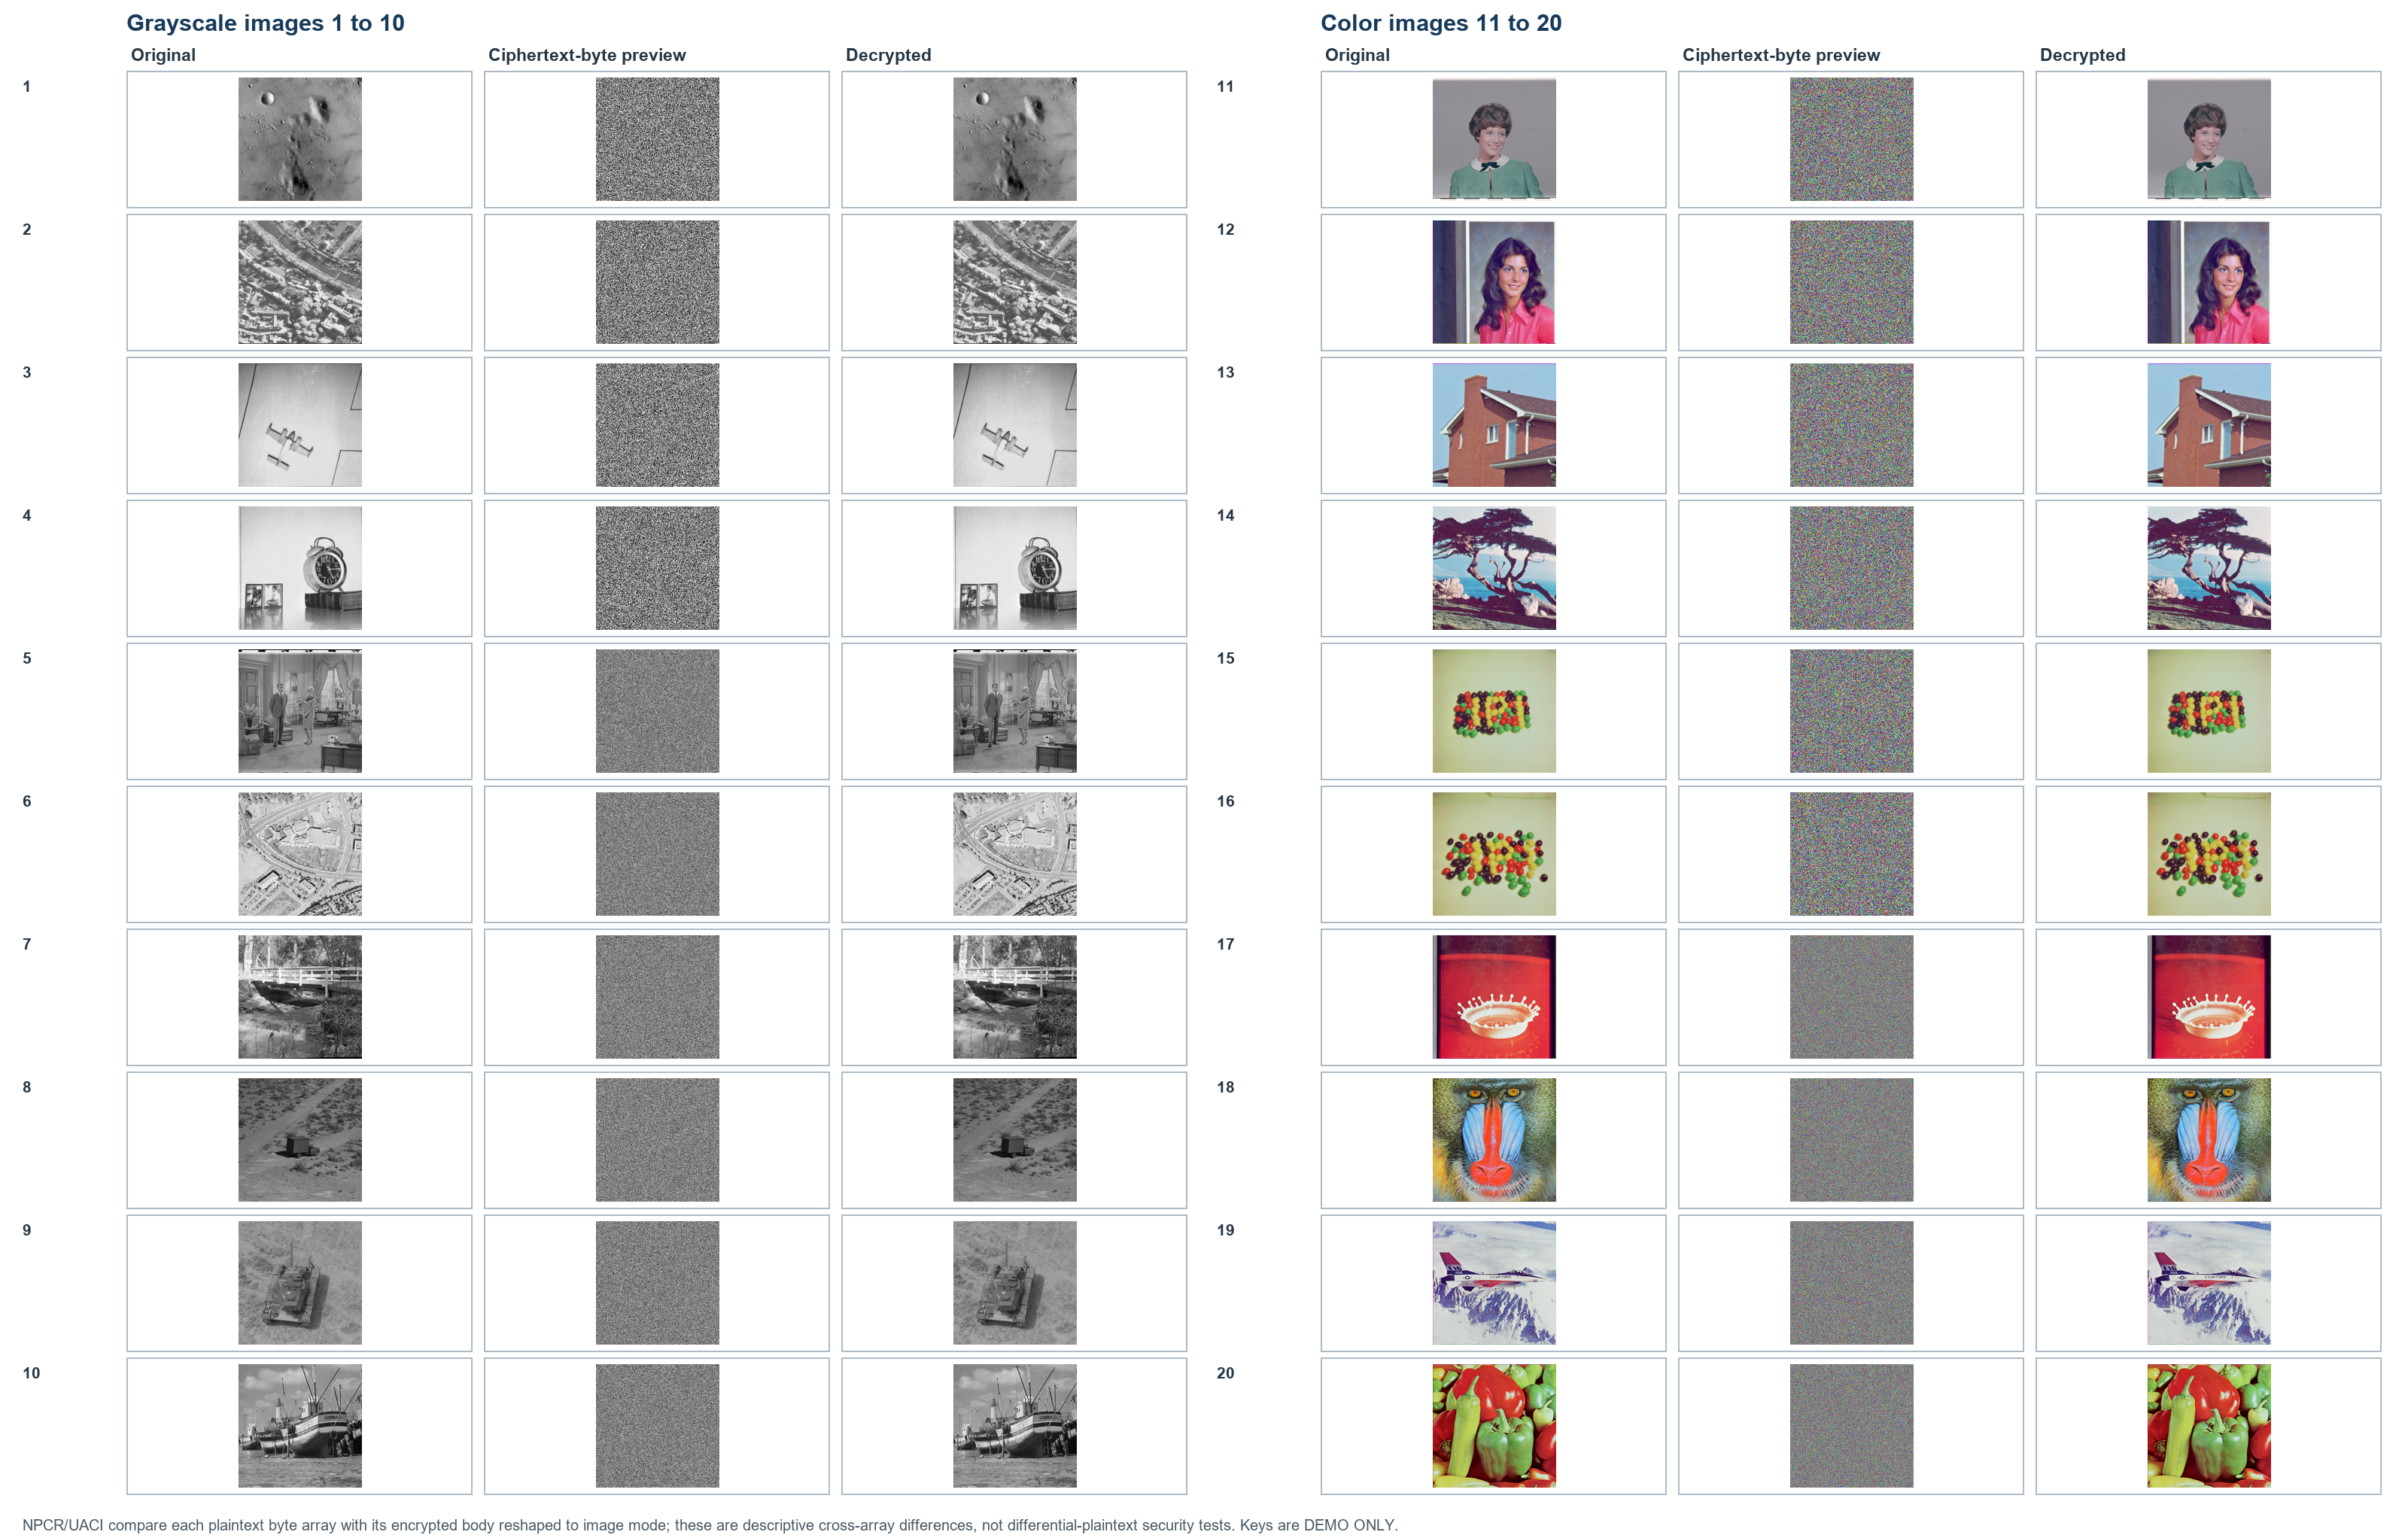
\includegraphics[width=0.99\textwidth]{figures/image_comparison_montage.png}
\caption{AES-256-GCM control results for all 10 grayscale and 10 color USC-SIPI images: original, ciphertext-byte preview, and exact decryption. All 20 decrypted pixel arrays matched their originals. The middle panels are visualization-only; each encrypted artifact is a binary authenticated container. Source images are from USC-SIPI \cite{uscSipi}; reproduction rights must be confirmed before submission.}
\label{fig:image-montage}
\end{figure*}

\begin{table*}[!t]
\caption{Per-image byte diagnostics for the 20 displayed AES-256-GCM control examples. $H(P)$, $H(C)$, and $H(D)$ are byte entropies of original pixels, ciphertext-body bytes, and recovered pixels. $NPCR(P,C)$ and $UACI(P,C)$ directly compare aligned original and ciphertext-body bytes; these are descriptive byte-array differences, not conventional differential tests comparing encryptions of $P$ and modified $P'$.}
\label{tab:per-image-metrics}
\centering\small
\setlength{\tabcolsep}{4pt}\renewcommand{\arraystretch}{1.05}
\begin{tabular}{rlrrrrrc}
\toprule
Image & Mode & $H(P)$ & $H(C)$ & $H(D)$ & $NPCR(P,C)$ (\%) & $UACI(P,C)$ (\%) & Exact \\
\midrule
1 & Gray & 6.709 & 7.997 & 6.709 & 99.585 & 26.201 & Yes \\
2 & Gray & 7.312 & 7.997 & 7.312 & 99.579 & 28.474 & Yes \\
3 & Gray & 6.452 & 7.997 & 6.452 & 99.596 & 33.453 & Yes \\
4 & Gray & 6.706 & 7.997 & 6.706 & 99.606 & 35.569 & Yes \\
5 & Gray & 7.201 & 7.999 & 7.201 & 99.625 & 27.588 & Yes \\
6 & Gray & 6.994 & 7.999 & 6.994 & 99.590 & 31.744 & Yes \\
7 & Gray & 5.706 & 7.999 & 5.706 & 99.621 & 29.949 & Yes \\
8 & Gray & 6.027 & 7.999 & 6.027 & 99.599 & 26.824 & Yes \\
9 & Gray & 5.496 & 7.999 & 5.496 & 99.643 & 26.207 & Yes \\
10 & Gray & 7.191 & 7.999 & 7.191 & 99.625 & 28.514 & Yes \\
11 & Color & 5.971 & 7.999 & 5.971 & 99.631 & 26.881 & Yes \\
12 & Color & 7.427 & 7.999 & 7.427 & 99.602 & 29.676 & Yes \\
13 & Color & 7.069 & 7.999 & 7.069 & 99.629 & 29.530 & Yes \\
14 & Color & 7.537 & 7.999 & 7.537 & 99.619 & 31.885 & Yes \\
15 & Color & 6.583 & 7.999 & 6.583 & 99.596 & 30.643 & Yes \\
16 & Color & 6.853 & 7.999 & 6.853 & 99.613 & 30.284 & Yes \\
17 & Color & 7.243 & 8.000 & 7.243 & 99.615 & 33.961 & Yes \\
18 & Color & 7.762 & 8.000 & 7.762 & 99.603 & 29.947 & Yes \\
19 & Color & 6.664 & 8.000 & 6.664 & 99.595 & 32.609 & Yes \\
20 & Color & 7.670 & 8.000 & 7.670 & 99.615 & 32.264 & Yes \\
\bottomrule
\end{tabular}
\end{table*}


\begin{table*}[!t]
\caption{Per-image fresh-nonce NPCR/UACI diagnostics for all 22 control assets. For each algorithm, the first pair compares two encryptions of the same plaintext; the second pair compares encryptions of the original and a one-byte-modified plaintext. Each entry is the mean of five comparisons. Since each encryption uses a fresh nonce, these measurements include nonce-induced differences and are not intrinsic-diffusion estimates. Images 1--20 are the displayed corpus; 21--22 are derived grayscale controls.}
\label{tab:per-image-differential}
\centering\scriptsize
\setlength{\tabcolsep}{2.4pt}\renewcommand{\arraystretch}{1.08}
\resizebox{\textwidth}{!}{%
\begin{tabular}{rr*{8}{r}}
\toprule
& & \multicolumn{4}{c}{Same plaintext, independent fresh nonces} & \multicolumn{4}{c}{One-byte plaintext change, fresh nonces} \\
\cmidrule(lr){3-6}\cmidrule(lr){7-10}
Image & Mode & \multicolumn{2}{c}{AES-GCM} & \multicolumn{2}{c}{ChaCha20-Poly1305} & \multicolumn{2}{c}{AES-GCM} & \multicolumn{2}{c}{ChaCha20-Poly1305} \\
\cmidrule(lr){3-4}\cmidrule(lr){5-6}\cmidrule(lr){7-8}\cmidrule(lr){9-10}
& & NPCR & UACI & NPCR & UACI & NPCR & UACI & NPCR & UACI \\
\midrule
1 & Gray & 99.61 & 33.49 & 99.62 & 33.46 & 99.61 & 33.47 & 99.60 & 33.45 \\
2 & Gray & 99.60 & 33.41 & 99.61 & 33.43 & 99.61 & 33.47 & 99.60 & 33.46 \\
3 & Gray & 99.59 & 33.41 & 99.59 & 33.39 & 99.60 & 33.49 & 99.61 & 33.48 \\
4 & Gray & 99.61 & 33.49 & 99.59 & 33.48 & 99.60 & 33.43 & 99.61 & 33.43 \\
5 & Gray & 99.62 & 33.47 & 99.61 & 33.44 & 99.61 & 33.43 & 99.60 & 33.47 \\
6 & Gray & 99.62 & 33.49 & 99.61 & 33.45 & 99.62 & 33.49 & 99.62 & 33.49 \\
7 & Gray & 99.62 & 33.46 & 99.61 & 33.47 & 99.61 & 33.45 & 99.60 & 33.43 \\
8 & Gray & 99.61 & 33.45 & 99.61 & 33.45 & 99.59 & 33.42 & 99.61 & 33.45 \\
9 & Gray & 99.61 & 33.49 & 99.62 & 33.48 & 99.60 & 33.45 & 99.61 & 33.46 \\
10 & Gray & 99.60 & 33.43 & 99.60 & 33.47 & 99.61 & 33.48 & 99.61 & 33.48 \\
11 & RGB & 99.61 & 33.46 & 99.61 & 33.44 & 99.60 & 33.45 & 99.61 & 33.44 \\
12 & RGB & 99.61 & 33.49 & 99.61 & 33.47 & 99.61 & 33.49 & 99.59 & 33.43 \\
13 & RGB & 99.60 & 33.48 & 99.61 & 33.48 & 99.61 & 33.42 & 99.60 & 33.47 \\
14 & RGB & 99.60 & 33.44 & 99.60 & 33.46 & 99.61 & 33.44 & 99.61 & 33.48 \\
15 & RGB & 99.62 & 33.43 & 99.61 & 33.42 & 99.61 & 33.43 & 99.61 & 33.49 \\
16 & RGB & 99.61 & 33.47 & 99.62 & 33.48 & 99.61 & 33.46 & 99.61 & 33.46 \\
17 & RGB & 99.60 & 33.46 & 99.61 & 33.47 & 99.61 & 33.45 & 99.61 & 33.45 \\
18 & RGB & 99.61 & 33.47 & 99.61 & 33.48 & 99.61 & 33.48 & 99.60 & 33.47 \\
19 & RGB & 99.61 & 33.45 & 99.61 & 33.46 & 99.61 & 33.45 & 99.60 & 33.46 \\
20 & RGB & 99.61 & 33.46 & 99.61 & 33.46 & 99.61 & 33.47 & 99.61 & 33.46 \\
21 & Gray & 99.61 & 33.48 & 99.61 & 33.46 & 99.61 & 33.45 & 99.62 & 33.46 \\
22 & Gray & 99.61 & 33.48 & 99.61 & 33.46 & 99.61 & 33.47 & 99.62 & 33.47 \\
\bottomrule
\end{tabular}%
}
\end{table*}

\begin{figure*}[!t]
\centering
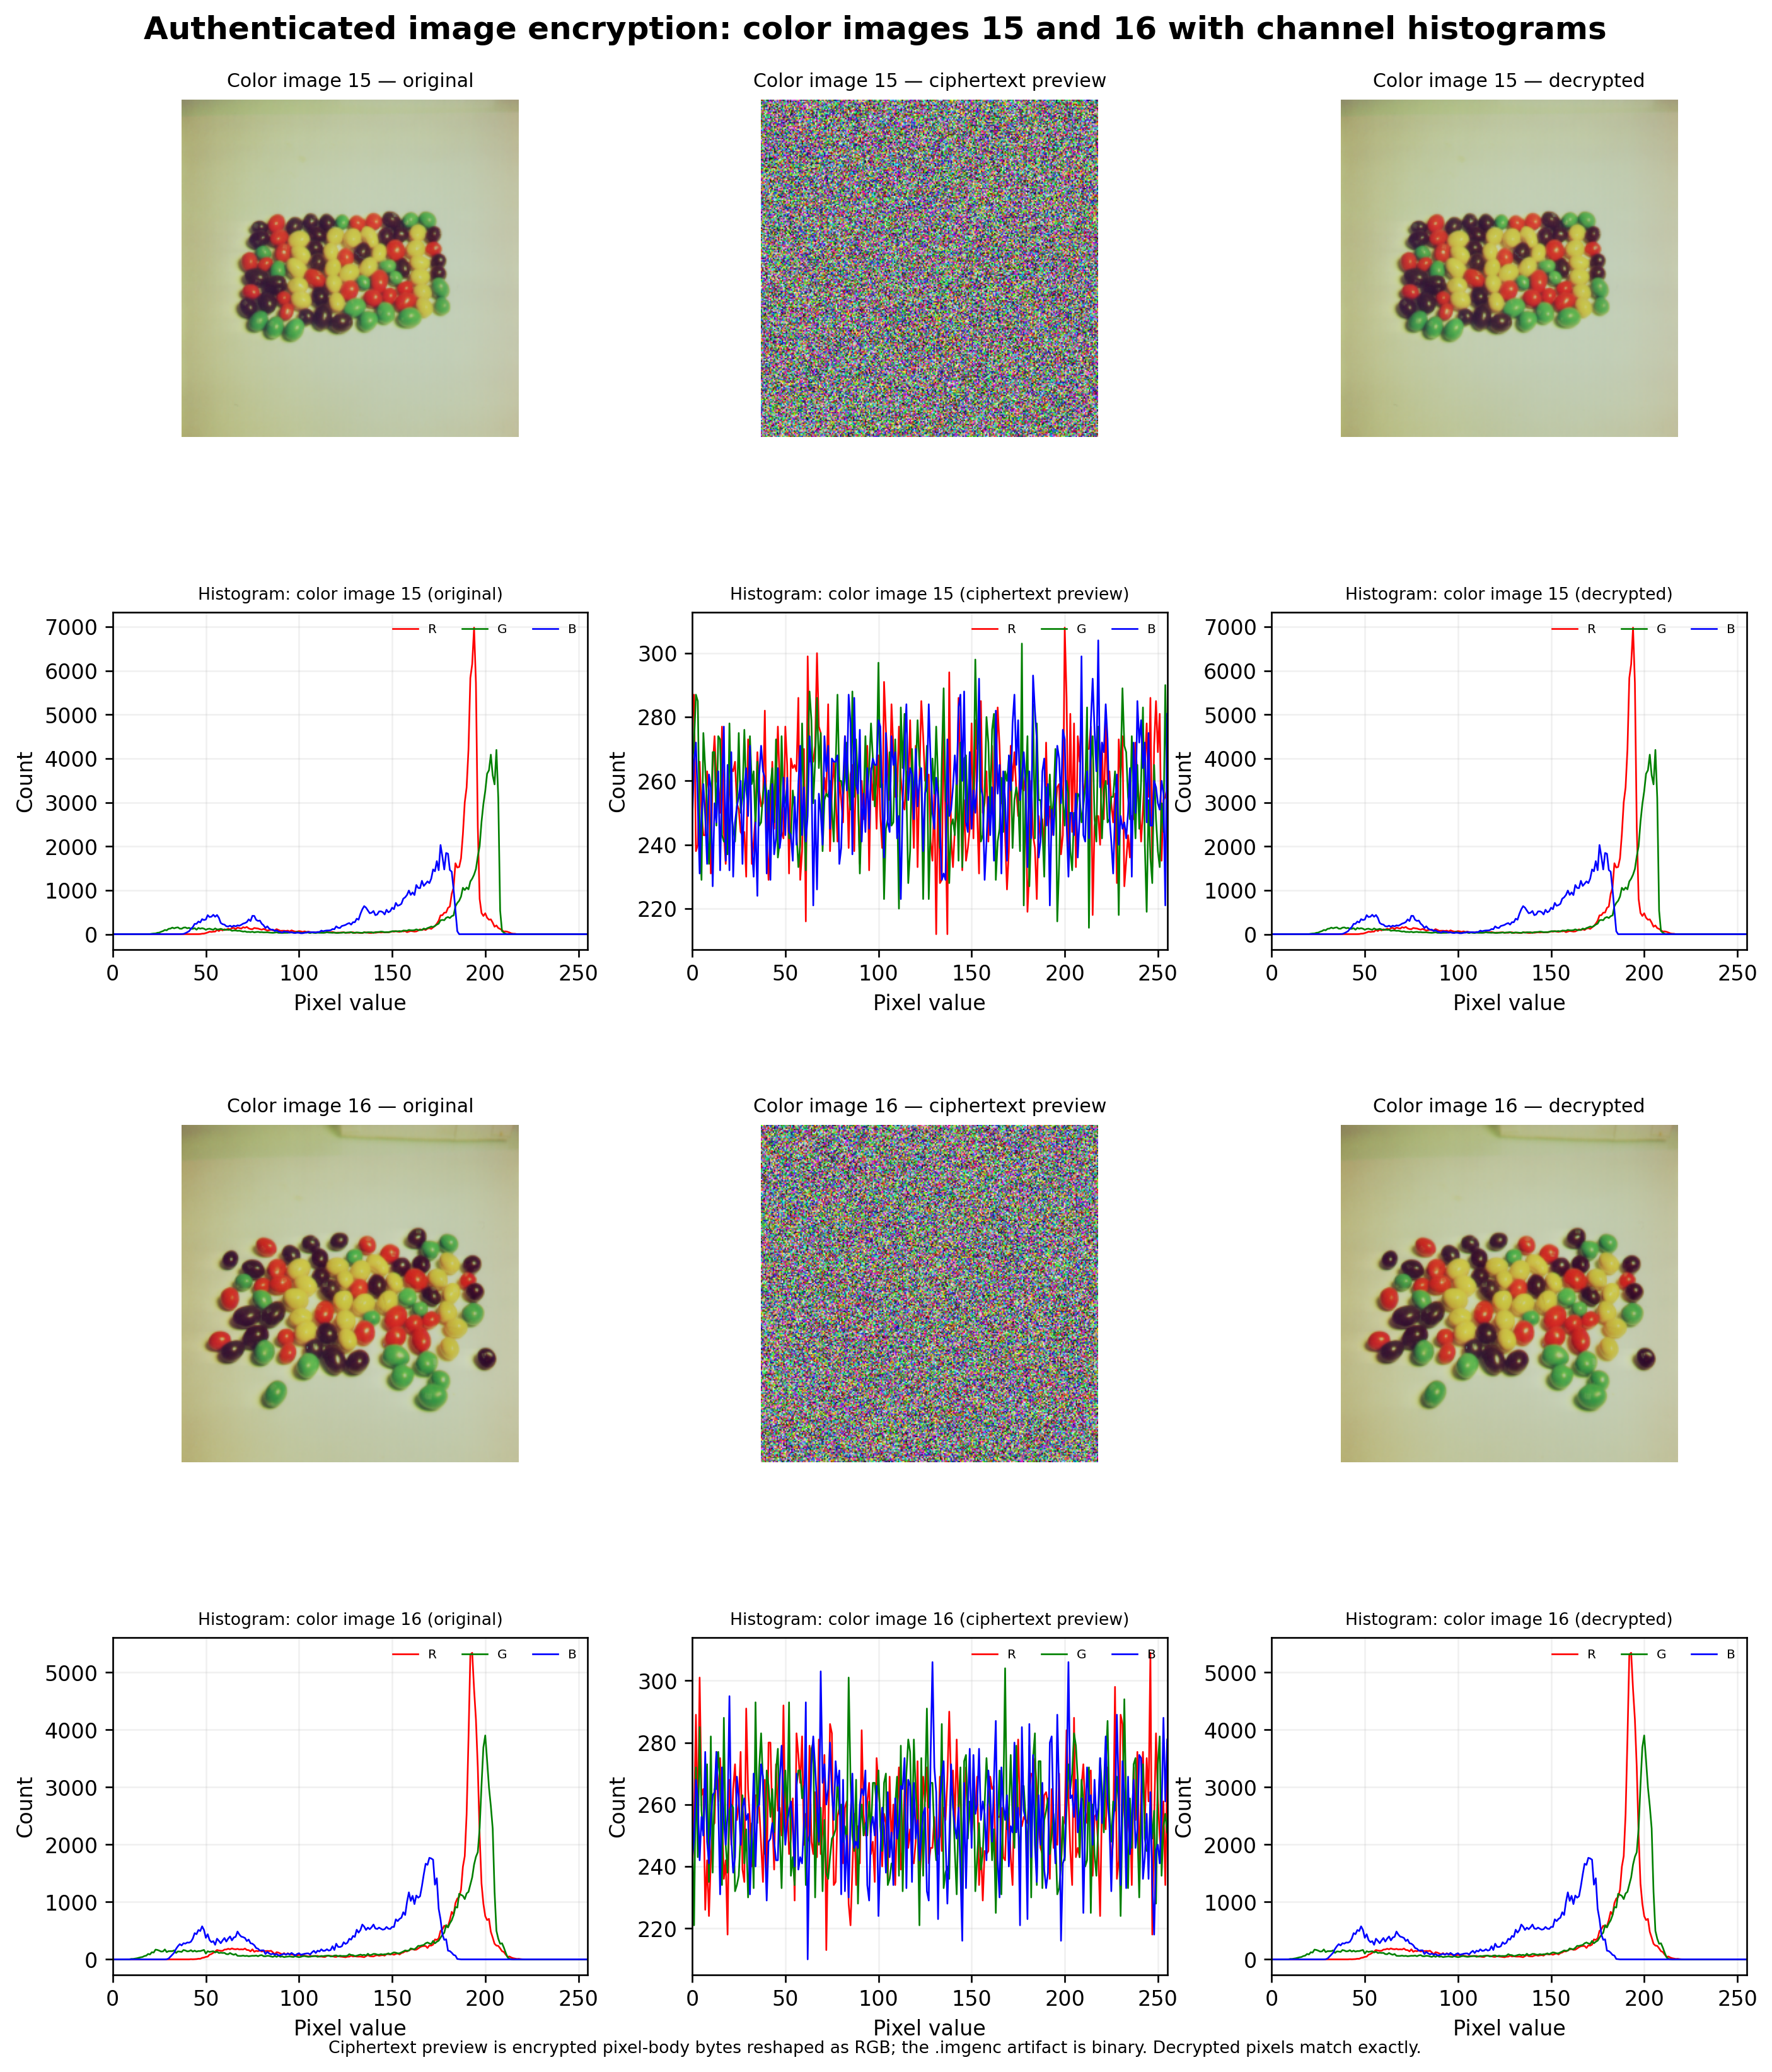
\includegraphics[width=0.96\textwidth]{figures/color_original_ciphertext_decrypted_histograms.png}
\caption{Color images 15 and 16. Each image row shows the original, ciphertext-byte display, and exact decryption; the following row shows the corresponding RGB-channel histograms. The source identifiers are retained in the image manifest. Ciphertext previews are not decryptable image files: the encrypted artifact is a binary authenticated container.}
\label{fig:color-demo}
\end{figure*}

\begin{figure*}[!t]
\centering
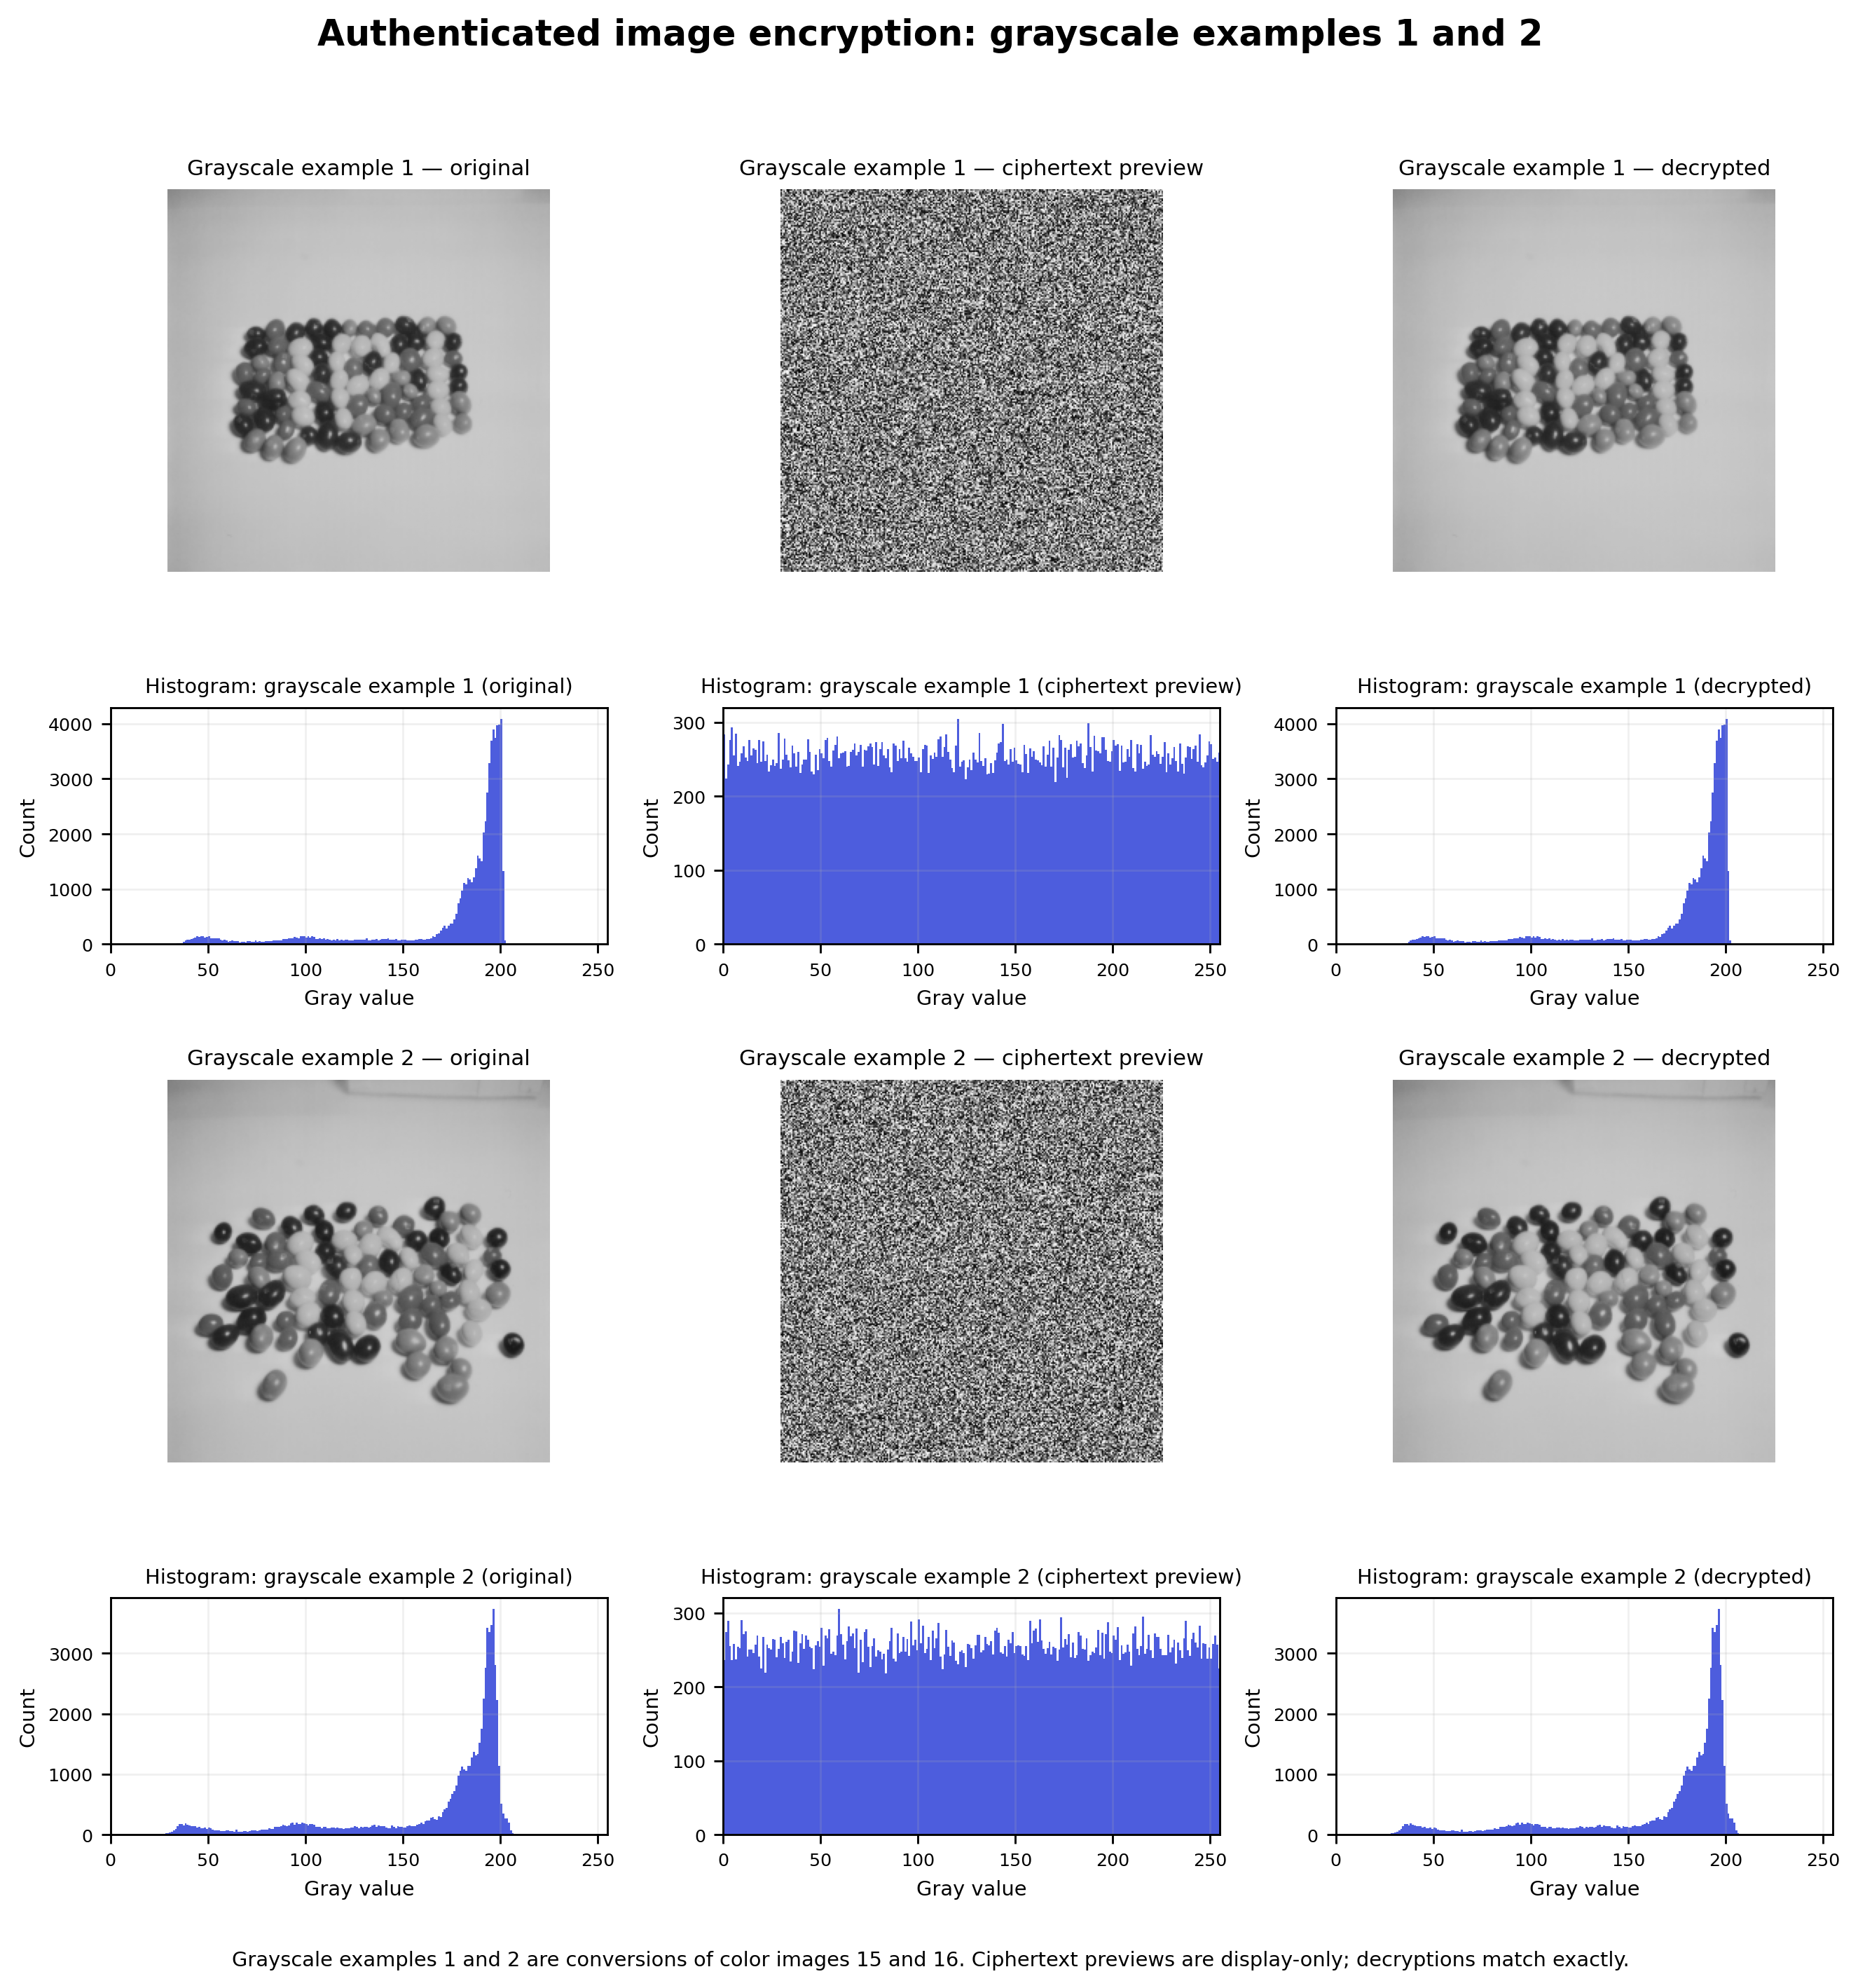
\includegraphics[width=0.96\textwidth]{figures/grayscale_original_ciphertext_decrypted_histograms.png}
\caption{Grayscale examples 1 and 2, derived from color images 15 and 16, respectively. Each row shows the original, ciphertext-byte display, and exact decryption, followed by the corresponding grayscale histograms. The middle panel is a visualization of encrypted pixel bytes, not a normal image ciphertext file.}
\label{fig:gray-demo}
\end{figure*}

On the four file cases using color images 15 and 16 (two images by two algorithms; 30 file-operation repetitions each), mean per-case median seal time was 3.97 ms and mean open-plus-PNG time was 25.61 ms. These measurements include codec and file operations and apply only to 256$\times$256 RGB images on the recorded machine. They are not directly comparable to the prior 22-image timing suite or to the six papers.

The image labels in Fig.~\ref{fig:image-montage} use simple serial numbers: 1--10 are grayscale and 11--20 are color. Table~\ref{tab:per-image-metrics} gives plaintext, ciphertext-body, and recovered byte entropy plus direct plaintext-to-ciphertext NPCR/UACI for every image. Because these compare different byte representations, those two columns are descriptive and must not be interpreted as conventional differential sensitivity scores. Table~\ref{tab:per-image-differential} reports separate, controlled five-pair fresh-nonce comparisons for all 22 assets and both AEAD algorithms, split between unchanged and one-byte-modified plaintext. It shows that near-ideal NPCR/UACI values occur in both conditions and therefore cannot isolate plaintext sensitivity in this setup.

For a concrete integrity demonstration, we re-opened each of the 20 saved binary containers and performed four probes: one authentication-tag bit flip, 1\% ciphertext-body byte corruption, 1\% truncation, and a one-bit wrong key. All 80/80 probes returned an authentication failure and produced no image. Fig.~\ref{fig:attack-evidence} shows representative grayscale image 1 and color image 11. The disclosed demonstration keys are only for reproducibility and must not be reused.

\begin{table*}[!t]
\caption{Detailed outcomes of the additional AEAD-control attack diagnostics. The observations refer to the standard reference algorithms and the specified harness only; they are not attack results against the six source-paper ciphers.}
\label{tab:attack-outcomes}
\centering\small
\setlength{\tabcolsep}{4pt}\renewcommand{\arraystretch}{1.12}
\begin{tabular}{p{0.16\textwidth}p{0.17\textwidth}p{0.23\textwidth}p{0.35\textwidth}}
\toprule
Probe & Work performed & Observed result & Interpretation \\
\midrule
Integrity/tamper & 572 mutation, metadata, truncation, and wrong-key probes across 44 image--algorithm cases & 572/572 rejected; no corrupted plaintext returned & Confirms fail-closed behavior for these tested inputs; not a general implementation proof. \\
Noise and reordering & 13 probes per each of four color-image/algorithm cases, including salt-and-pepper and Gaussian noise at 0.1, 1, 5, and 10\%, byte changes, metadata, truncation, and block reordering & 52/52 rejected & AEAD detects modification; it does not provide graceful recovery from ciphertext damage. \\
CPA distinguisher & 500 randomized challenges per image--algorithm case; two RGB images & 242--265 correct of 500 (48.4--53.0\%); every Wilson 95\% interval includes 50\% & No advantage was detected by this one simple classifier; this is not an IND-CPA proof. \\
KPA transfer & One known pair, then 100 fresh-nonce target messages per case & 0/100 target prefixes recovered in each of four cases & A bounded cross-nonce transfer probe; not a general key-recovery result. \\
Wrong-key sensitivity & 100 random wrong keys per case, plus one-bit key changes & 400/400 random-key attempts rejected; all one-bit changes rejected & Authentication failure is expected for AEAD and does not quantify key sensitivity of the six custom ciphers. \\
Ciphertext-only diagnostics & Byte entropy, histograms, channel statistics, and spatial correlation & Ciphertext statistics were measured; no plaintext/key-recovery attempt was made & Statistical descriptions alone do not constitute a COA. \\
Timing screen & 1,500 fixed-size samples per input class and algorithm; Welch test & AES-GCM: $p=0.361$; ChaCha20-Poly1305: $p=0.455$ & Exploratory and inconclusive; neither a nonsignificant result nor this sample establishes constant-time behavior. \\
Brute force / scrambling-only & No exhaustive key search; no separate permutation layer exists in AEAD & No brute-force result; scrambling-only is not applicable & For an ideal 256-bit key, expected exhaustive search is $2^{255}$ trials; this is a theoretical estimate, not measured work. \\
\bottomrule
\end{tabular}
\end{table*}

\begin{figure*}[!t]
\centering
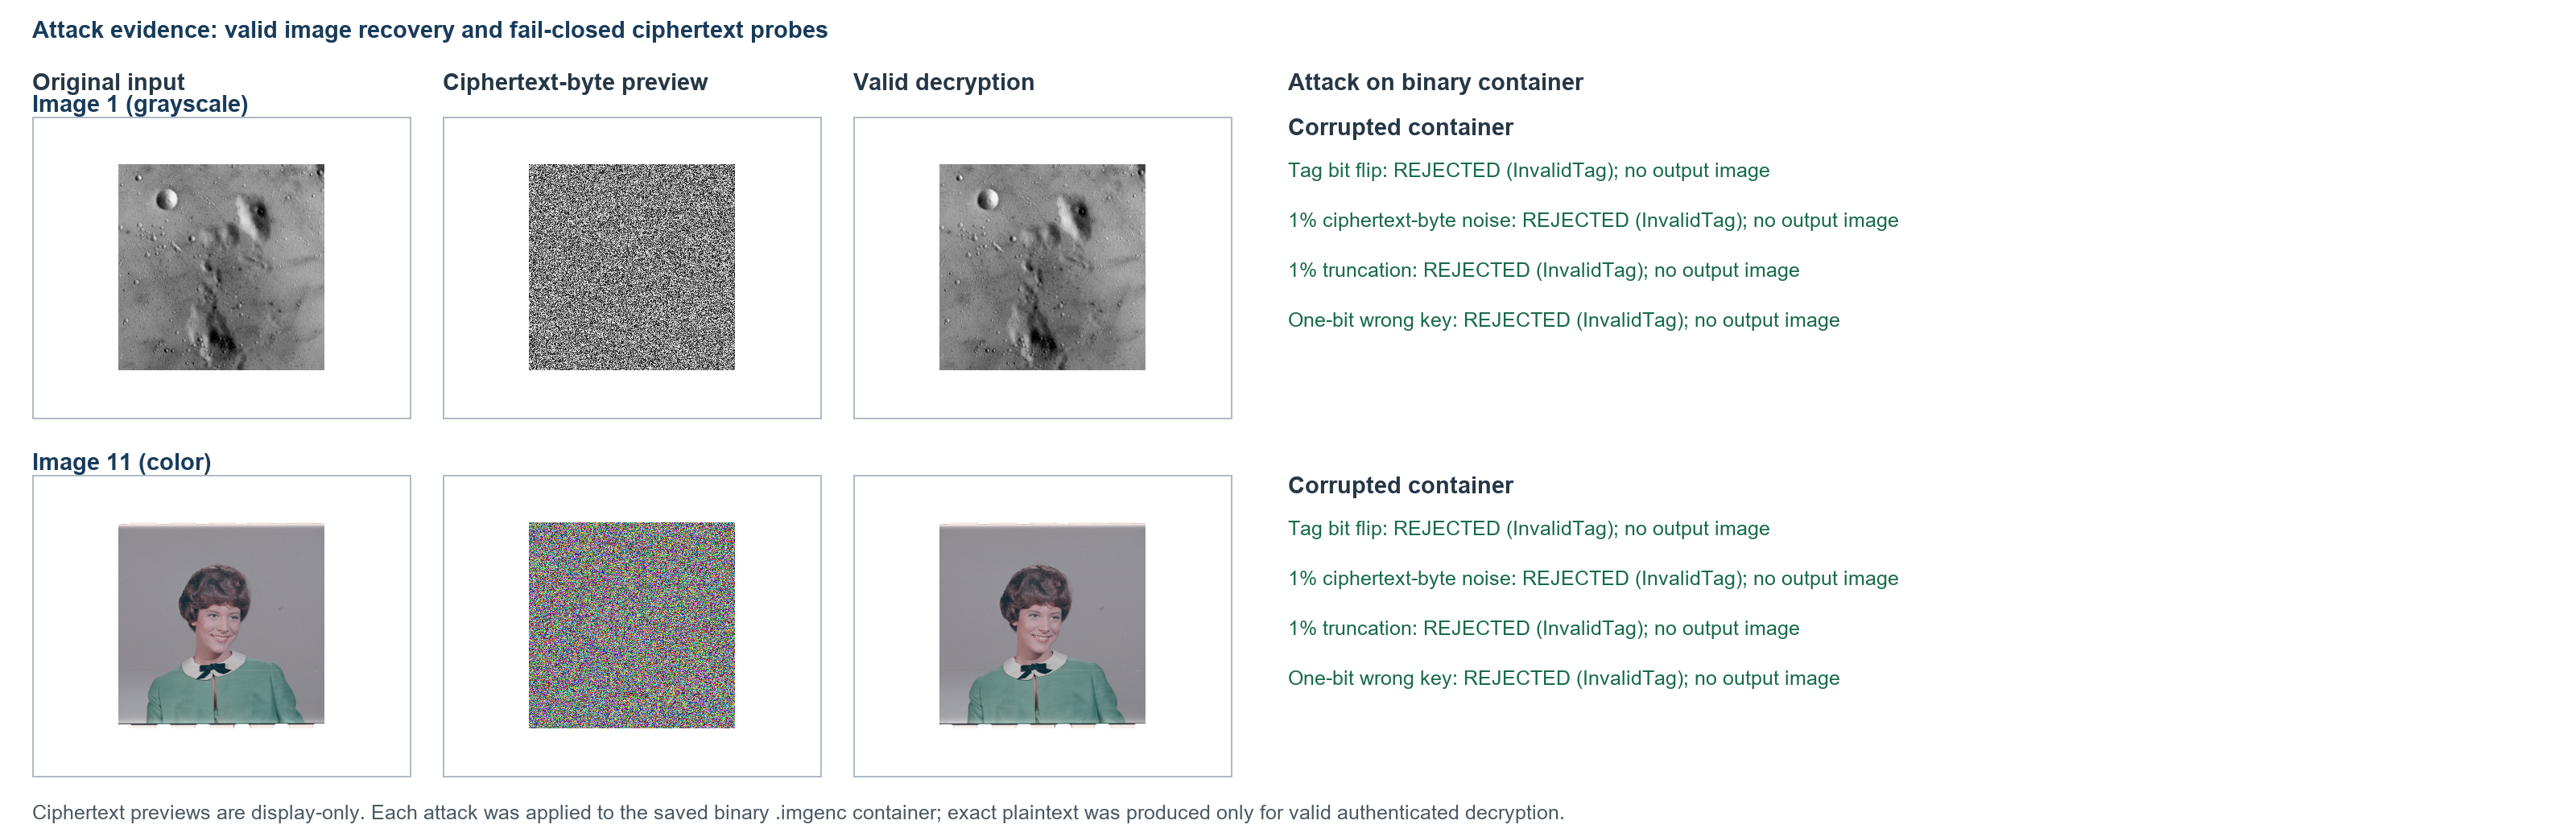
\includegraphics[width=0.98\textwidth]{figures/attack_evidence.png}
\caption{Representative fail-closed attack probes for grayscale image 1 and color image 11. Valid containers decrypt exactly; tag changes, ciphertext-byte noise, truncation, and a one-bit wrong key are rejected, so no output image is emitted. The tested binary containers use disclosed demonstration keys and are not secure keys.}
\label{fig:attack-evidence}
\end{figure*}

The source-paper coverage matrix is in Table~\ref{tab:attack-matrix}; “claim only” marks a claim in a source paper without a direct recovery experiment. Table~\ref{tab:attack-outcomes} gives concrete counts and observed outcomes for the additional CPA, KPA-transfer, ciphertext-only diagnostic, noise/tampering, wrong-key, brute-force, scrambling-only, and timing probes on the reference controls. For the controls, the measured CPA, KPA-transfer, ciphertext-only statistics, noise/tampering, wrong-key, and exploratory timing results are reported here and in Table~\ref{tab:controls}. Scrambling-only testing is not applicable because the AEAD container has no independent pixel-permutation stage. The two-image CPA classifier was correct on 242--265 of 500 challenges per case (48.4\%--53.0\%); each Wilson 95\% interval included 50\%. Across these color-image cases, byte entropy ranged from 7.9989 to 7.9991 bits, and mean absolute spatial correlation ranged from 0.0025 to 0.0038. Fresh-nonce NPCR/UACI was 99.608--99.610\%/33.457--33.474\% for unchanged plaintext and 99.605--99.609\%/33.456--33.468\% for one-byte-changed plaintext. The tested KPA transfer probe recovered 0 of 100 target prefixes in each case. All 13 mutation/noise/reordering probes, 100/100 wrong keys, and the one-bit key change were rejected per case. These outcomes describe these particular probes only. The exploratory timing screen found no statistically significant class difference in this rerun (AES-GCM $p=0.361$; ChaCha20-Poly1305 $p=0.455$). A previous exploratory run had yielded an AES-GCM $p=0.0246$, which did not reproduce. This variation shows that the current screen is too noisy for a side-channel conclusion; neither run establishes an exploitable leak or constant-time behavior. The nominal 256-bit key-space estimate is a mathematical assumption, not a measured brute-force result.

The following tables answer two different comparison questions: reported image-statistic results across the six source papers, and which attacks each paper actually tested. Published values are transcribed from the supplied PDFs. They are not a controlled ranking because image sets, channels, plaintext edits, key/nonce rules, and implementations differ. “NR” means not reported in the supplied paper; it does not mean a failed test.

\begin{table*}[!t]
\caption{Reported statistics and attack tests in the six supplied papers. Reported inputs and protocols differ, so values should not be ranked as a controlled benchmark.}
\label{tab:literature-metrics}
\centering
\small
\begin{tabular}{p{0.15\textwidth}p{0.23\textwidth}p{0.24\textwidth}p{0.32\textwidth}}
\toprule
Paper & Ciphertext entropy & NPCR/UACI (\\%) & Other reported tests and caveats \\\\
\midrule
Niu et al. \cite{niu2024} & 7.9970--7.9973 (5 grayscale) & Mean 99.6082 / 33.4733 (5 images) & Histogram, $\chi^2$, correlation, key sensitivity, noise and cropping recovery; not direct CPA/KPA/COA. \\\\
Zhang et al. \cite{zhang2024} & 7.9617--7.9915 (reported entries) & Lena 99.6093 / 33.4635; Baboon 99.8046 / 33.3984 & Histogram, correlation, Fourier, key sensitivity, salt-pepper/cutting tests; reported runtime uses a separate MATLAB/PC setup. \\\\
Zhu and Zhu \cite{zhu2024} & Near 8 bits (paper-reported) & NR & Histogram, correlation, feature-code/noise robustness, and a CPA resistance claim; visual-security carrier embedding differs from ordinary cipher arrays. \\\\
Yan et al. \cite{yan2025} & 7.9992--7.9993 per RGB channel & NR & Histogram, channel correlation, key sensitivity, noise and cropping recovery. \\\\
Geng et al. \cite{geng2025} & About 7.9968--7.9994 (local-entropy table) & Mean 99.6184 / 33.4734 (7 images) & Histogram, local entropy, floating frequency, noise and clipping recovery; local entropy is not global entropy. \\\\
Al-Dayel et al. \cite{aldayel2025} & About 7.9977 (reported mean) & Mean 99.6143 / 33.4983 (8 images) & Histogram, chi-square, key sensitivity; CPA/KPA/brute-force claims are not direct recovery tests. Noise/occlusion is applied before encryption. \\\\
\bottomrule
\end{tabular}
\end{table*}

Table~\ref{tab:literature-metrics} makes the requested entropy and NPCR/UACI comparison explicit. The reported values cluster near the usual image-statistic targets, as summarized in Fig.~\ref{fig:literature-npcr-uaci}; the inputs and protocols differ. In particular, NPCR/UACI values calculated with different images, edits, and nonce behavior cannot establish that one cipher is stronger. Our fresh-nonce AEAD controls are therefore reported separately in Table~\ref{tab:controls}; the near-identical scores for unchanged and edited plaintexts show why those values alone are not an attack result.

\begin{figure*}[!t]
\centering
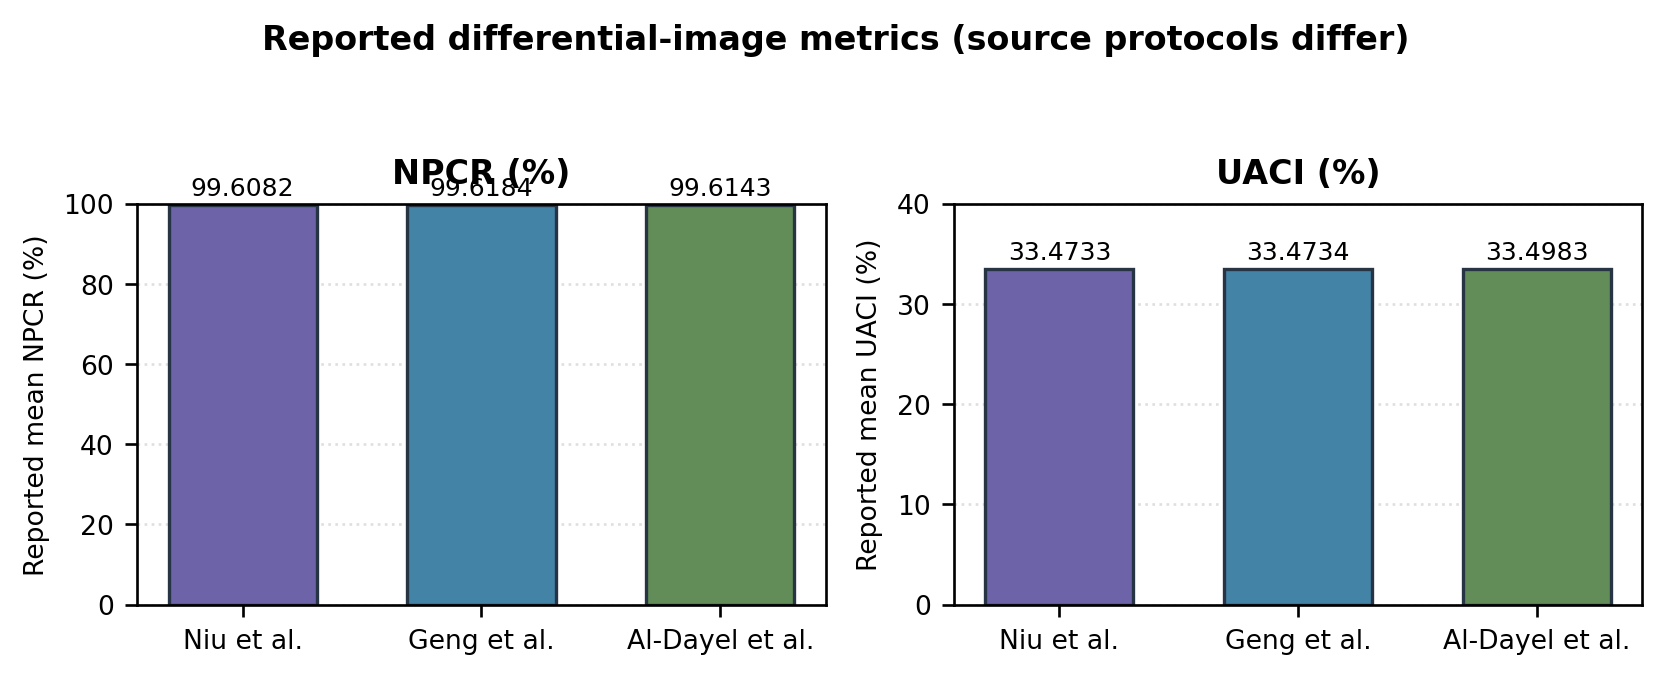
\includegraphics[width=0.95\textwidth]{figures/reported_npcr_uaci_comparison.png}
\caption{Mean NPCR/UACI recalculated from the image-level tables reported by Niu et al., Geng et al., and Al-Dayel et al. \cite{niu2024,geng2025,aldayel2025}. The underlying image sets, perturbations, and protocols differ; this descriptive plot is not a controlled ranking.}
\label{fig:literature-npcr-uaci}
\end{figure*}




\begin{table*}[!t]
\caption{Coverage of reported tests in the six supplied papers and tests run on our separate AEAD controls.}
\label{tab:attack-matrix}
\centering
\small
\setlength{\tabcolsep}{3pt}
\renewcommand{\arraystretch}{1.22}
\begin{tabular}{p{1.14in}*{6}{>{\centering\arraybackslash}p{0.48in}}p{2.12in}}
\toprule
Test & Niu & Zhang & Zhu & Yan & Geng & Al-Dayel & Our AEAD controls \\
\midrule
NPCR/UACI & M & M & NR & NR & M & M & P--C diagnostics; fresh-nonce pairs \\
Histogram & S & S & S & S & S & S & Per-image histogram and $\chi^2$ \\
Entropy & S & S & S & S & S & S & Plaintext, ciphertext, and recovered images \\
Correlation & S & S & S & S & S & S & Horizontal/vertical pixel correlation \\
Noise/cropping recovery & R & R & R & R & R & R$^7$ & Corruption rejected; no recovery claimed \\
CPA & NR & NR & C & NR & NR & C & 500-challenge diagnostic \\
KPA & NR & NR & NR & NR & NR & C & 100-target transfer diagnostic \\
COA & NR & NR & NR & NR & NR & NR & Ciphertext-only statistics only \\
Timing/runtime & NR & T & T & NR & O & O & In-memory and file-wrapper timing \\
Brute force/key sensitivity & K & K & K & K & K & K & 256-bit keys; wrong-key probes \\
Scrambling-only & NR & NR & NR & NR & NR & NR & Not applicable to AEAD \\
\bottomrule
\end{tabular}
\vspace{1mm}
\parbox{\textwidth}{\scriptsize M: image-difference metric; S: statistical analysis; R: corruption/noise recovery; C: security claim without direct key/content recovery; T: measured runtime; O: asymptotic complexity only; K: key-space or key-sensitivity discussion; NR: not reported. Our AEAD column describes separate controls, not tests of the six custom ciphers. Al-Dayel et al. corrupt the image before encryption.}
\end{table*}

The matrix reports each paper's tests separately from this study's AEAD controls and equation-level audits. Noise/cropping recovery and cryptographic attack resistance answer different questions: recovering a visually recognizable image after partial damage does not show resistance to CPA/KPA/COA, while AEAD rejection of changed bytes provides integrity but intentionally does not reconstruct damaged plaintext. For that reason, we do not label image-statistic tests as successful attacks or claim that the AEAD controls break the six custom schemes.

\begin{table}[!t]
\caption{Summary of the AEAD control run.}
\label{tab:controls}
\centering
\small
\resizebox{\columnwidth}{!}{%
\begin{tabular}{lrr}
\toprule
Measure & AES-256-GCM & ChaCha20-Poly1305 \\
\midrule
Exact round trips & 22/22 & 22/22 \\
Rejected probes & 286/286 & 286/286 \\
Byte entropy (bits/byte) & 7.99894 & 7.99895 \\
Mean absolute correlation & 0.00214 & 0.00240 \\
Same-image NPCR/UACI (\%) & 99.609/33.461 & 99.609/33.457 \\
Changed-image NPCR/UACI (\%) & 99.609/33.457 & 99.608/33.461 \\
Mean per-image median encryption time (ms) & 0.161 & 0.252 \\
Mean per-image median decryption time (ms) & 0.155 & 0.249 \\
Mean encryption throughput (MiB/s) & 2,022.02 & 1,239.89 \\
Mean decryption throughput (MiB/s) & 1,917.66 & 1,212.49 \\
\bottomrule
\end{tabular}%
}
\end{table}

\begin{table}[!t]
\caption{File-level wrapper measurements across 22 images (mean of per-image values; nine repetitions per case).}
\label{tab:file-timing}
\centering
\small
\resizebox{\columnwidth}{!}{%
\begin{tabular}{lrrrr}
\toprule
Algorithm & PNG level & Seal (MiB/s) & Open + PNG (MiB/s) & Mean PNG bytes \\
\midrule
AES-256-GCM & 6 & 75.00 & 8.20 & 191,071 \\
AES-256-GCM & 1 & 78.55 & 11.45 & 276,159 \\
ChaCha20-Poly1305 & 6 & 74.23 & 8.37 & 191,071 \\
ChaCha20-Poly1305 & 1 & 74.30 & 10.62 & 276,159 \\
\bottomrule
\end{tabular}
}
\end{table}

\subsection{Seed-Equation Availability Finding}
Eleven of the 12 grayscale images produced defined seeds. Image 5.1.09 did not: its four XOR aggregates were $[224,223,0,8]$, so one denominator was zero. Among the 10,000 one-pixel variants of image 4.2.03, 161 (1.61\%) produced at least one zero aggregate. The Wilson 95\% interval for this probe proportion is 1.38\%--1.88\%. Under a simplifying model of four independent uniform byte aggregates, the expected probability is $1-(255/256)^4=1.553\%$. The observed result is consistent with that simple model. It shows an input-dependent definedness problem in the written seed formula; it does not show a confidentiality break.

\begin{figure}[!t]
\centering
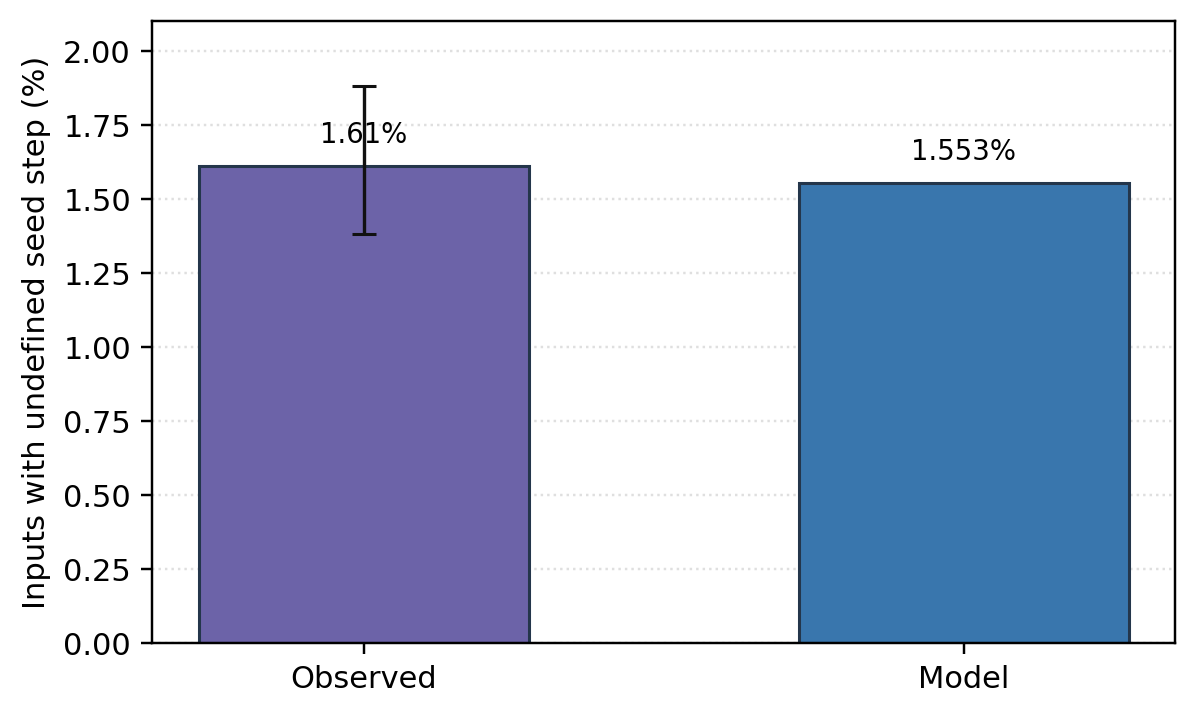
\includegraphics[width=0.88\columnwidth]{figures/seed_equation_availability.png}
\caption{Observed zero-denominator rate among 10,000 one-pixel chosen-input probes (1.61\%) and expected value under an independent-uniform model for four byte aggregates (1.553\%). The Wilson 95\% interval for the observed proportion is 1.38\%--1.88\%.}
\label{fig:seed-audit}
\end{figure}

\begin{table}[!t]
\caption{Real-domain check of Zhu and Zhu Eqs. (20)--(21) on one million uniform input pairs.}
\label{tab:zhu-domain}
\centering
\small
\begin{tabular}{lrr}
\toprule
Event & Observed & Expected \\
\midrule
Negative $Z_1$ radicand & 49.9928\% & 50\% \\
Negative $Z_2$ radicand & 49.9651\% & 50\% \\
At least one negative & 75.0047\% & 75\% \\
\bottomrule
\end{tabular}
\end{table}

\subsection{Reproduction Status of the Six Papers}
The control suite applies generic image and integrity diagnostics, but it does not run the proposed algorithms in the six papers. The Zhang equation audit does identify a non-injective mapping in the stated cyclic-XOR diffusion: for the documented example bit-plane grouping, two distinct chosen plaintexts yield identical diffusion outputs and hence identical later deterministic ciphertexts. This establishes a decryption-correctness failure under the published equations, but does not amount to key recovery or plaintext recovery. For Geng et al., direct PDF inspection found forward steps without inverse steps, an equation/prose conflict, and no stated ODE solver or step size. For Zhu and Zhu, the printed Box--Muller equations have negative radicands over much of the stated domain, and matrix construction is not uniquely specified. For Yan et al., Eq. (10) has an ambiguous channel-sum expression and decryption is described only at a high level. These remaining findings block faithful end-to-end reproduction without assumptions.



\section{Discussion}
The results illustrate a basic measurement problem. NPCR/UACI values near their often-cited targets can result from randomized nonces even when the plaintext has not changed. Therefore, these values are not enough to show resistance to differential cryptanalysis. Likewise, near-eight-bit entropy, low neighboring-pixel correlation, and a passing histogram threshold describe sample arrays but do not replace an attacker model.

AEAD controls provide a different kind of evidence: they bind the ciphertext to a key and metadata and reject changes in this test suite. The probes are basic integrity checks, not proof that our test harness or a new scheme is secure. The throughput figures also depend on implementation and machine details. A fair performance comparison requires the target ciphers and baselines to use the same hardware, software versions, image bytes, warm-up, and timing boundaries.

The Niu and Geng findings both concern plaintext-dependent initialization. In Niu et al., the published equations use the plaintext hash and column means, but the receiver procedure is only described as an inverse and does not explain how it obtains these inputs. For Geng et al., the zero-denominator condition makes the written seed equation undefined for some valid inputs; an implementation could add a fallback, but that would change the published method and require separate evaluation. Neither schedule finding demonstrates plaintext recovery.

The Zhu and Zhu equations show a separate reproducibility problem. As printed, Eqs. (20)--(21) do not produce real Gaussian values over much of the stated input domain. The subsequent matrix-construction and SVD description also repeats placeholder-like notation in the published PDF. These findings support a request for clarification or code release. They do not prove that the authors' implementation used the equations literally or that its cipher is insecure.

\section{Limitations and Required Work}
This is a pilot study. No custom cipher from the six papers has been independently implemented end to end. The Niu audit covers only its seed equations; the 1,000 chosen inputs are not a CPA against the full cipher. We have not run genuine chosen-plaintext or chosen-ciphertext attacks, key-recovery attempts, exhaustive search, or a scheme-specific NIST sequence evaluation against any target cipher. The AEAD probes are controls and must not be presented as attacks against the six papers. The image corpus is small, and its rights status is uncertain for many files. Runtime results use one machine and cannot be ranked against the published results. File-level measurements include PNG serialization and are much lower than in-memory cipher throughput; they do not establish improved speed against the papers.

Before this manuscript can support a TIFS submission, the work needs: (1) independent reproductions of selected schemes; (2) published inputs, outputs, exact numeric settings, and implementations; (3) explicit attacker models and successful or bounded direct attack attempts; (4) matched runtime and memory comparisons; (5) rights-cleared data or suitable replacement assets; (6) a complete citation and authorship review; and (7) a fresh check of current TIFS author requirements. Publication in a Q1 journal cannot be guaranteed by formatting or by a target choice.

\section{Conclusion}
We audited the reported tests of six recent chaos-based image-encryption papers and ran AES-256-GCM and ChaCha20-Poly1305 as reference controls on 22 grayscale and RGB images. The controls passed exact round trips and rejected all 572 basic corruption and wrong-key probes. Their near-ideal fresh-nonce NPCR/UACI values also appeared for unchanged plaintext, showing why image-difference statistics alone cannot establish cipher diffusion or attack resistance. Equation-level audits found input-dependent Niu initial states under 1,000 one-pixel probes, a perfect equality distinguisher under the stateless deterministic reading of Niu et al.'s published method, a zero denominator in the stated Geng seed equations for one corpus image and 161 of 10,000 probes, and a negative radicand in the printed Zhu and Zhu Box--Muller equations for about 75\% of the stated uniform input domain. The Niu distinguisher reveals equality only; it does not recover image contents or a key. No complete target cipher was reproduced, so the next step is an end-to-end implementation and additional direct cryptanalysis before any superiority claim.

\section*{Code and Data Availability}
The scripts, processed result files, and image manifest are provided in a separate reproducibility supplement for this draft. The USC-SIPI image files are not redistributed because reuse rights are uncertain for some selected images; the manifest gives the source identifiers, dimensions, and hashes. Before journal submission, the authors should deposit the code and eligible data in a persistent public repository, obtain a citable identifier, and replace this statement with the final repository link. The six source papers are identified by DOI in the reference list.

\section*{Acknowledgment}
\textit{Complete this section only if there are actual contributors or funding sources to acknowledge.}

\bibliographystyle{IEEEtran}
\bibliography{refs}
\end{document}
